
\documentclass[12pt,a4paper]{article}
\usepackage[left=2.5cm,right=2.5cm,top=1.0cm,bottom=2cm]{geometry}
%\documentclass{article}
\usepackage{graphicx}
\usepackage{subcaption}
\usepackage{amsmath}
\parindent=1cm
%\marginparwidth = 0pt
%\hoffset = 0pt
%\oddsidemargin = 0pt
%\marginparsep = 0pt
%\voffset = 0pt

%\documentclass{amsproc}
%\documentclass[11pt,
%paper=a4,
%bibtotocnumbered,	  % Literaturverzeichnis ins Inhaltsverzeichnis
%liststotocnumbered,  % Alle Listen ins Inhaltsverzeichnis							
%DIV=calc,		  % führt die Satzspiegelberechnung neu aus
%oneside,		  % einseitiger Druck
%tablecaptionabove,	  % Tabellenüberschriften aktivieren
%BCOR=16mm,	  % Bindekorrektur
%headinclude,
%footinclude
%]{article}

\usepackage{fancyhdr}
\usepackage{lipsum} % only for showing some sample text
\fancyhf{} % clear all header and footers
\renewcommand{\headrulewidth}{0pt} % remove the header rule

\rfoot{\thepage}
\pagestyle{fancy}
\usepackage{indentfirst} % Красная строка

\usepackage[utf8]{inputenc}
\usepackage{graphicx} %includegraphics
\usepackage{braket} %Bra and Ket
\usepackage{amsmath} %mathcal etc
\usepackage{natbib} %citep, citet, bib-style
\usepackage[colorlinks]{hyperref}
\newcommand{\mysubtitle}[1]{\section{#1}}
\usepackage[usenames,dvipsnames]{xcolor}
\definecolor{persianplum}{rgb}{0.44, 0.11, 0.11}
\definecolor{mulberry}{rgb}{0.77, 0.29, 0.55}
\definecolor{maroon(html/css)}{rgb}{0.5, 0.0, 0.0}
\definecolor{indigo(dye)}{rgb}{0.0, 0.25, 0.42}
\begin{document}
\title{$\pi$ - pulse}
\author{}
\date{\today}
\maketitle
\chapter{Dynamical repulsive-to-attractive conversion of interactions}
\label{chap:pi_pulse}
\section{Introduction}
The creation of a population inversion in metallic bands corresponding to a negative temperature state \citep{PhysRev.81.279,PhysRev.103.20} is one of the ways to control the interparticle interaction. Such investigation was done in the work of \citep{PhysRevB.85.155124} for hypercubic lattice, where it was shown that it is possible to induce the population inversion in metallic systems using properly shaped half-cycle or monocycle pulses, the system without energy dissipation will thermalize in the negative temperature state after the pulse. Effective switching of the interaction from repulsive to attractive occurs because a density matrix $\exp ({-H/T})$ for a Hamiltonian $H$ with temperature $T < 0$ corresponds inverted $-H$ with $-T > 0$ \citep{PhysRevLett.105.220405,PhysRevLett.106.236401}.

In this chapter, we rely on the work \citep{PhysRevB.85.155124} taking realistic 2D square lattice and focused on transient nonequilibrium dynamics with different polarization of the electric field.
By the half-cycle pulse, we induce a shift in the momentum distribution of the electrons. Selecting the parameters of such pulse we can achieve half of the Brillouin zone, the system is brought to the negative-$T$ state, this is often (depending on the value of the interaction) leads to change of the interaction from repulsive to attractive.

Below we provide calculations for 2D square lattice with hopping amplitude $t=1$, initial inverse temperature $\beta=1/T=5$ and $32 \times 32$ $k$-grid. Time has units of reverse hoppings. 
%\clearpage
\section{Population invertion induced by a linear polarized pulse}

To investigate the effects of negative temperature state we use a single-band Hubbard model driven by the half-cycle electric field. The half-cycle pulses with amplitude of vector potential ($A_{max}$) and pulse length ($\tau$) chosen in $Y$ and $XY$ (diagonal) polarisation directions.
%The vector potential has the form:
%\begin{equation}
%A(t)=\frac{A_{max}}{\tau}(t-\tau sin(2\pi t/\tau))
%\end{equation}
%where $A_{max}$ - amplitude of vector potential; $\tau$ - pulse length.
\begin{figure}[h!]
\begin{minipage}[h]{0.5\linewidth}
\center{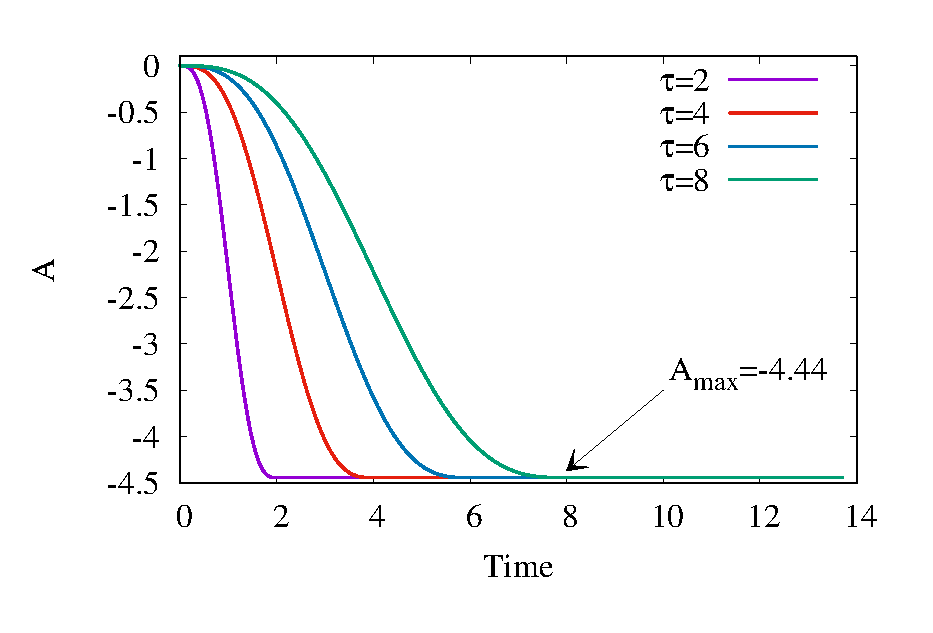
\includegraphics[width=1\linewidth]{Chapters/1_pi_pulse_tex/figure/xy/PulseA.eps}} (a) \\
\end{minipage}
\hfill
\begin{minipage}[h]{0.5\linewidth}
\center{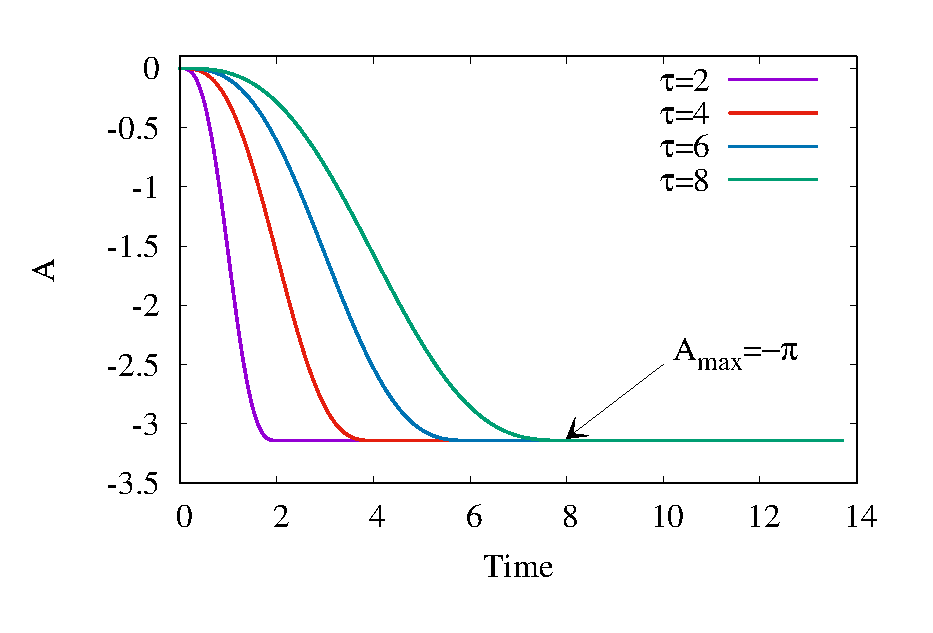
\includegraphics[width=1\linewidth]{Chapters/1_pi_pulse_tex/figure/y/PulseA.eps}} \\(b)
\end{minipage}
\begin{minipage}[h]{0.5\linewidth}
\center{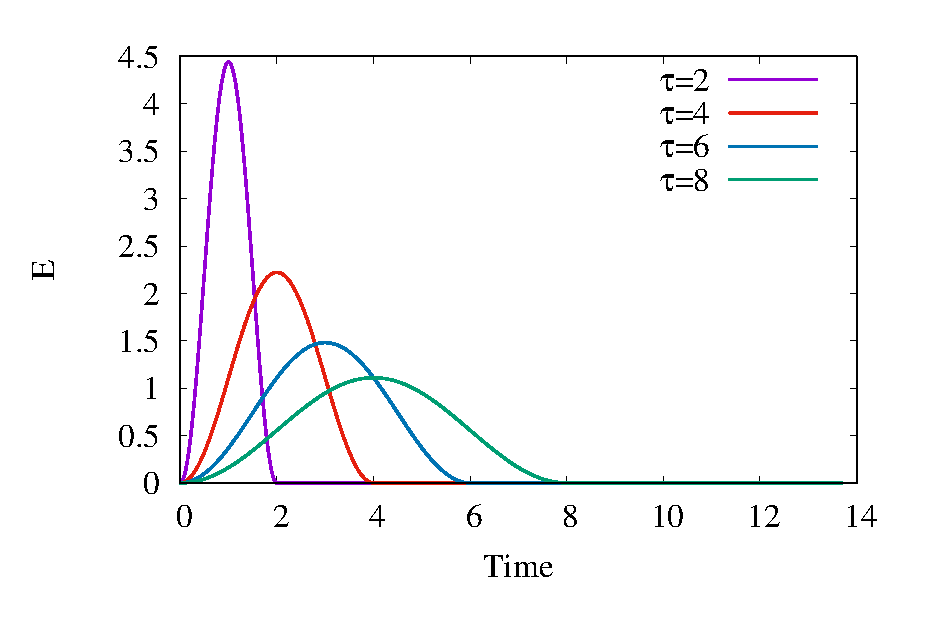
\includegraphics[width=1\linewidth]{Chapters/1_pi_pulse_tex/figure/xy/PulseE.eps}} (c) \\
\end{minipage}
\hfill
\begin{minipage}[h]{0.5\linewidth}
\center{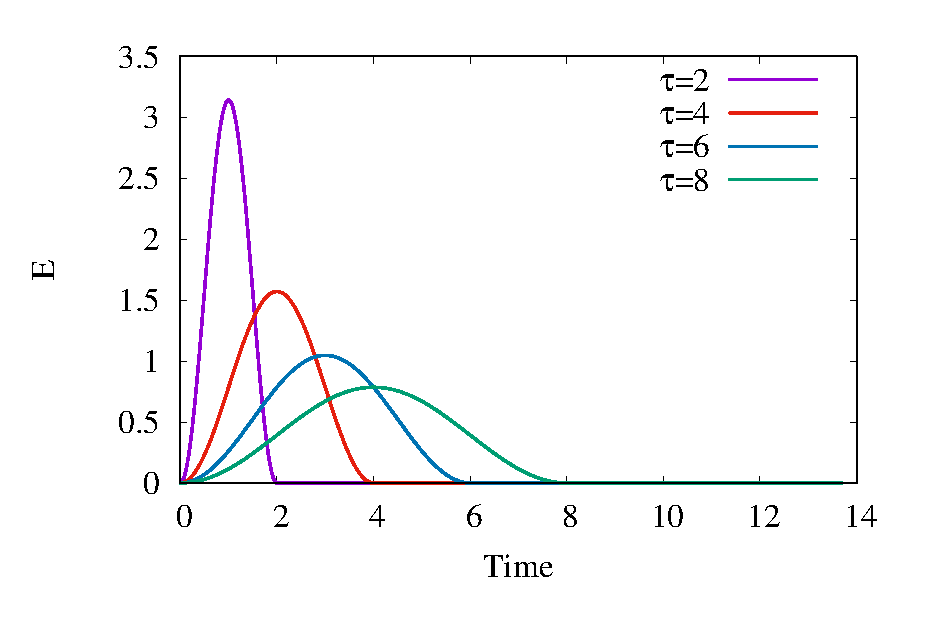
\includegraphics[width=1\linewidth]{Chapters/1_pi_pulse_tex/figure/y/PulseE.eps}} \\(d)
\end{minipage}
\caption{Vector potential and external electric field: (a),(c) for $XY$-polarization; (b),(d) for $Y$-polarization}
\label{fig:Pulses}
\end{figure}
In case of $Y$-polarization, the maximum value of the vector potential is as follows $A_{max} = \pi$ (Fig.~\ref{fig:Pulses}b). For diagonal polarization the maximum value of the vector potential $A_{max} =\pi*\sqrt{2}$ depicted in Fig.~\ref{fig:Pulses}a. The corresponding electric fields are shown in the Figs.~\ref{fig:Pulses}c,d. This allows to shift the momentum distribution in the case of $Y$-polarization from $\Gamma$ to Y, in the case of $XY$-polarization from $\Gamma$ to M in the Brillouin zone.

After the pulse excitation the isolated system strives to achieve a thermalized state with some effective temperature $T_{eff}$ and total energy $E_{tot}$. A thermal state with a positive temperature has $E_{tot} < 0$ at half filling, while $E_{tot} > 0$ happens at negative temperature ($T_{eff} < 0$). Thereby the total energy is an order parameter for the repulsion-to-attraction transition \citep{PhysRevB.85.155124}.

To show the effect of the population inversion we choose the half-cycle shape of the electric field with $\tau = 4$ (red line in Figs.~\ref{fig:Pulses}c,d) and investigate the behavior of the total energy and double occupancy (Fig.~\ref{fig:E_tot}).
\begin{figure}[h!]
\begin{minipage}[h]{0.5\linewidth}
\center{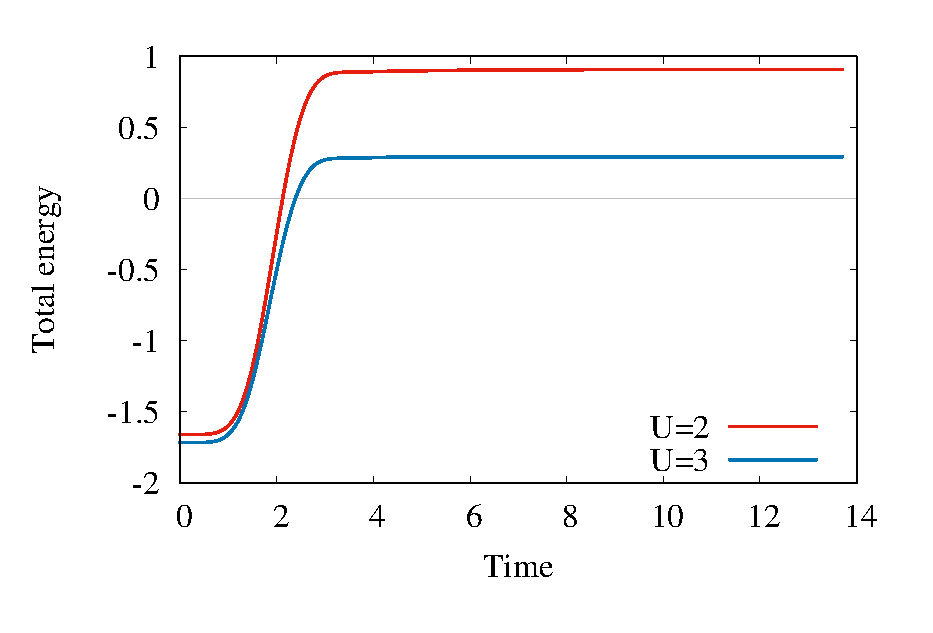
\includegraphics[width=1\linewidth]{Chapters/1_pi_pulse_tex/figure/xy/E_tot_xy.eps}} (a) \\
\end{minipage}
\hfill
\begin{minipage}[h]{0.5\linewidth}
\center{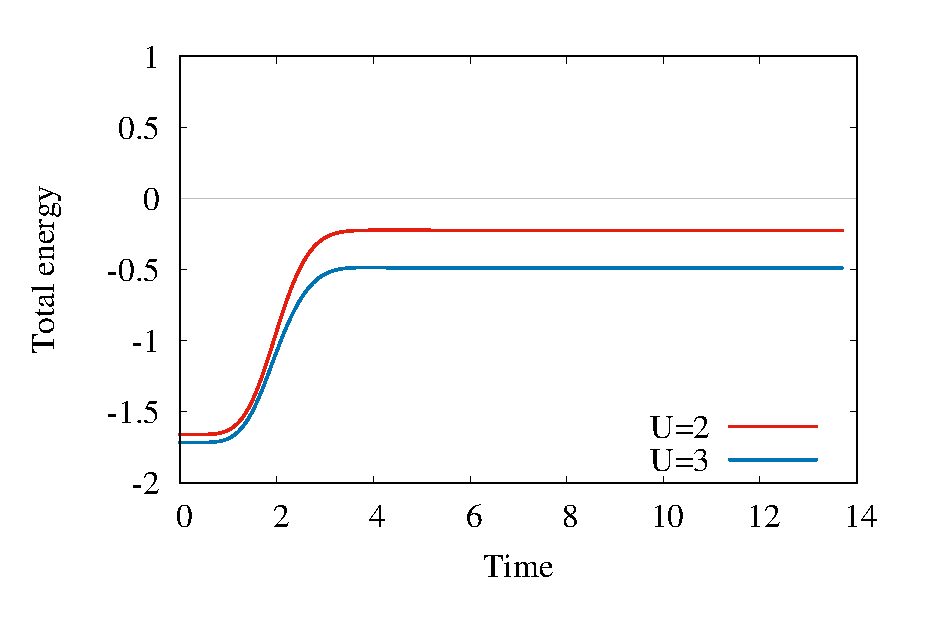
\includegraphics[width=1\linewidth]{Chapters/1_pi_pulse_tex/figure/y/E_tot_y.eps}} \\(b)
\end{minipage}
\begin{minipage}[h]{0.5\linewidth}
\center{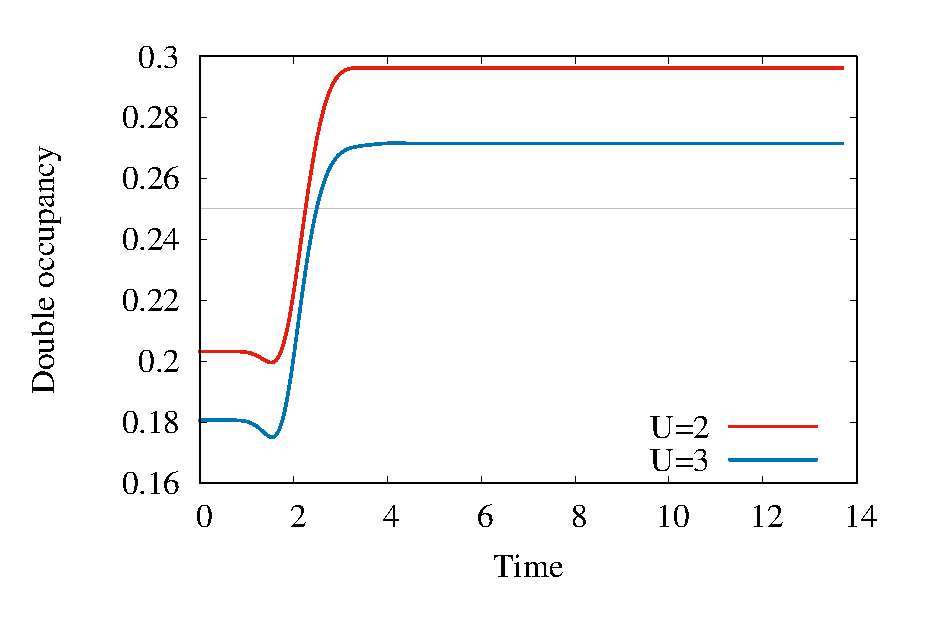
\includegraphics[width=1\linewidth]{Chapters/1_pi_pulse_tex/figure/xy/docc_xy.eps}} (c) \\
\end{minipage}
\hfill
\begin{minipage}[h]{0.5\linewidth}
\center{\includegraphics[width=1\linewidth]{Chapters/1_pi_pulse_tex/figure/y/docc_y.eps}} \\(d)
\end{minipage}
\caption{Total energy and double occupancy ($\tau = 4$): (a),(c) for $XY$ direction of pulse polarization ($A_{max} =\pi\sqrt{2}$); (b),(d) for $Y$-polarization ($A_{max} = \pi$).}
\label{fig:E_tot}
\end{figure}

From the analysis of Figs.~\ref{fig:E_tot}a,c we can observe a change in the sign of the interaction in case of field in the $XY$-polarization, $U=2$ and $U=3$. $E_{tot}>0$ (the total energy has the origin at zero) and the double occupancy $docc>0.25$ after the pulse. Then lower Coulomb interaction than $E_{tot}$ has a bigger value and a more pronounced effect of the negative temperature state after the pulse. In the case of $Y$-polarization of the electric field, the total energy negative all the time, so the interaction does not change the sign.
\begin{figure}[h!]
\center{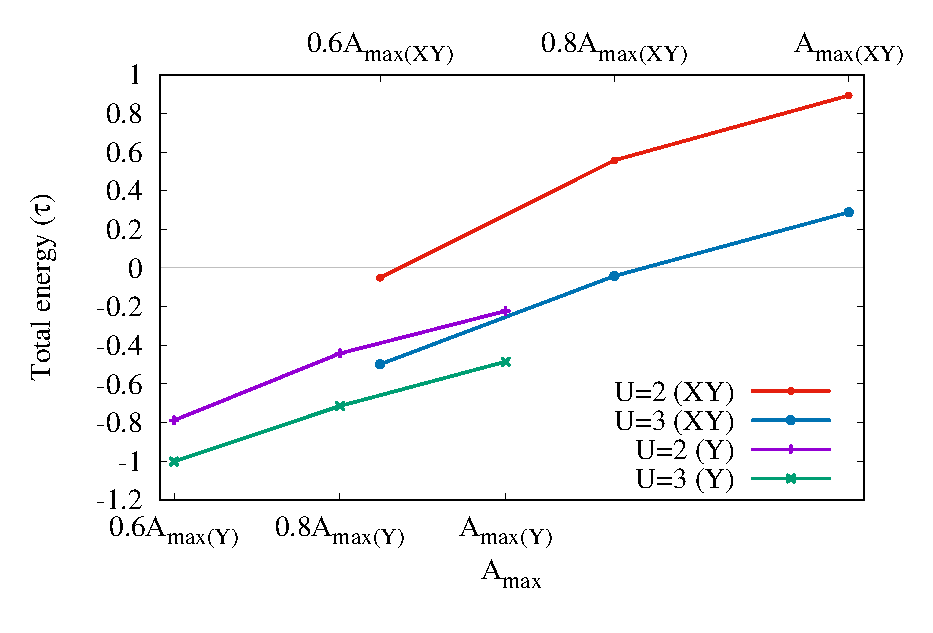
\includegraphics[width=0.7\linewidth]{Chapters/1_pi_pulse_tex/figure/xy/E_mpi.eps}} \\
\caption{The total energy after the pulse as a function of the magnitude of the vector potential ($\tau = 4$).}
\label{fig:E_tot_A}
\end{figure}

In the Fig.~\ref{fig:E_tot_A} is shown the total energy after the pulse for $\tau=4$ as a function of the magnitude of the vector potential for both polarizations. For the field in $XY$-polarization, there is positive total energy, which means that the sign of interaction has changed. The value of the total energy is maximum when the value of the amplitude of the vector potential such that exactly shift momentum distribution in the case of $Y$-polarization from $\Gamma$ to Y points in the Brillouin zone and the case of $XY$-polarization from $\Gamma$ to M. The value of the total energy decreases with increasing $U$. In the case of $Y$-polarization, there is no change in the sign of the interaction for all values of the vector potential and the Coulomb interaction. These statements are consistent with the results of the article \citep{PhysRevB.85.155124}.
\begin{figure}[h!]
\center{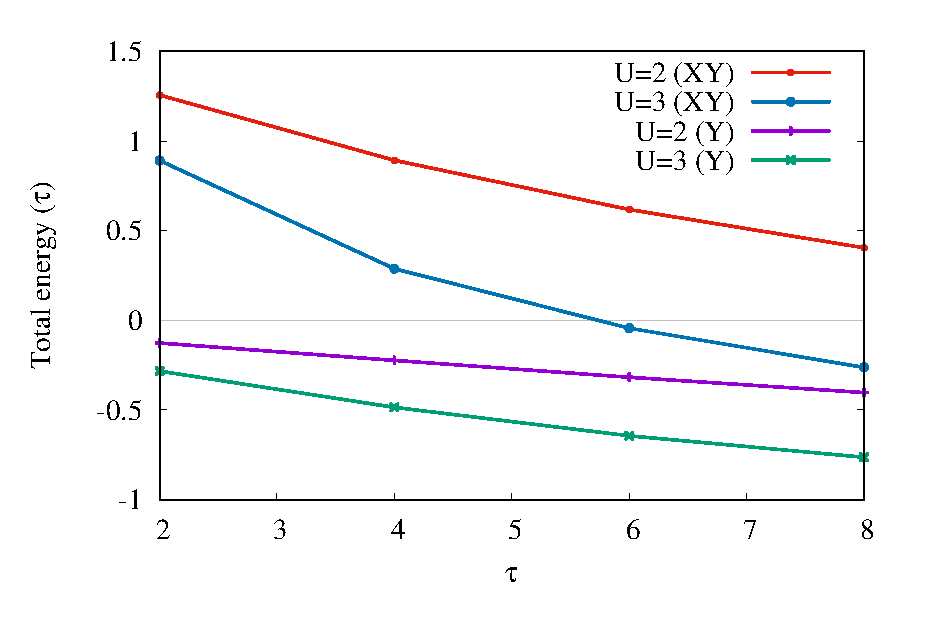
\includegraphics[width=0.7\linewidth]{Chapters/1_pi_pulse_tex/figure/xy/E_tau.eps}} \\
\caption{The total energy after the pulse as a function of the pulse width.}
\label{fig:E_tot_tau}
\end{figure}
%\clearpage

The total energy after the half-cycle pulse as a function of pulse width depicted in Fig.~\ref{fig:E_tot_tau}. For the pulse with $\tau = 2$ ($XY$-polarization), the total energy has a positive and maximum value (red and blue lines), this pulse narrowest in the calculations. With increasing pulse width, the total energy after the pulse can become negative, as seen on the blue line. This behavior was also demonstrated in the work \citep{PhysRevB.85.155124} for the hypercubic lattice.
In the case of a pulse in the $Y$-polarization, the total energy is always negative. With increasing pulse width, the total energy goes deep into the negative region.
%\subsection{Modification of momentum distribution under half-cycle linear polarized pulse.}

Visually change of an electron population can be traced in the time-dependent momentum distribution. Fig.~\ref{fig:md_u2_t0} shows the momentum distribution of the interacting system ($U=2$) at time $t=0$ when the system is in equilibrium and the field does not affect it.
\begin{figure}[h!]
\center{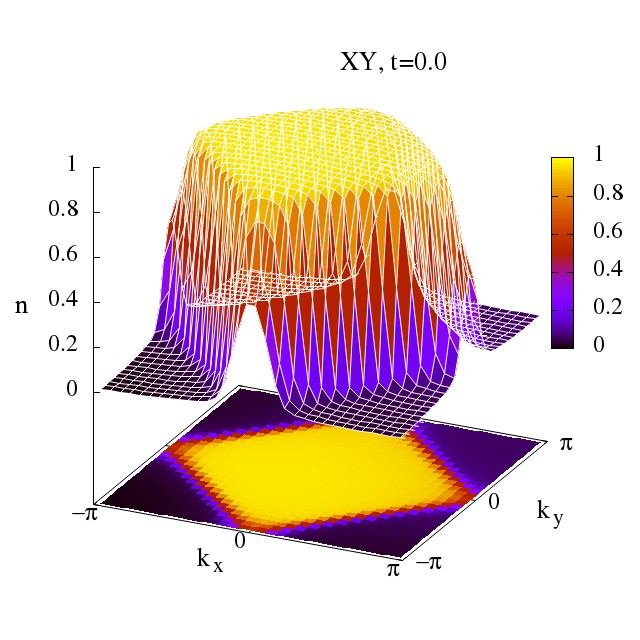
\includegraphics[width=0.5\linewidth]{Chapters/1_pi_pulse_tex/figure/y/A_0.jpg}} \\
\caption{Equilibrium momentum distribution for $U=2$ at $time=0$.}
\label{fig:md_u2_t0}
\end{figure}

\begin{figure}[hp]
\begin{minipage}[h]{0.43\linewidth}
\begin{overpic}[width=1\textwidth]{Chapters/1_pi_pulse_tex/figure/xy/u2/A_200.jpg}
 \put (20,85) {(a)}
\end{overpic}
\end{minipage}
\hfill
\begin{minipage}[h]{0.43\linewidth}
\begin{overpic}[width=1\textwidth]{Chapters/1_pi_pulse_tex/figure/y/u2/A_200.jpg}
 \put (20,85) {(b)}
\end{overpic}
\end{minipage}
\begin{minipage}[h]{0.43\linewidth}
\begin{overpic}[width=1\textwidth]{Chapters/1_pi_pulse_tex/figure/xy/u2/A_300.jpg}
 \put (20,85) {(c)}
\end{overpic}
\end{minipage}
\hfill
\begin{minipage}[h]{0.43\linewidth}
\begin{overpic}[width=1\textwidth]{Chapters/1_pi_pulse_tex/figure/y/u2/A_300.jpg}
 \put (20,85) {(d)}
\end{overpic}
\end{minipage}
\begin{minipage}[h]{0.43\linewidth}
\begin{overpic}[width=1\textwidth]{Chapters/1_pi_pulse_tex/figure/xy/u2/A_400.jpg}
 \put (20,85) {(e)}
\end{overpic}
\end{minipage}
\hfill
\begin{minipage}[h]{0.43\linewidth}
\begin{overpic}[width=1\textwidth]{Chapters/1_pi_pulse_tex/figure/y/u2/A_400.jpg}
 \put (20,85) {(f)}
\end{overpic}
\end{minipage}
\caption{Momentum distribution for $U=2$ at different $time$ $\in$ [2,4], $\tau=4$. Left column (a),(c),(e) - field in $XY$-polarization; right column (b),(d),(f) - field in $Y$-polarization.}
\label{fig:md_u2_A_max}
\end{figure}
%\clearpage



\begin{figure}[hp]
\begin{minipage}[h]{0.43\linewidth}
\begin{overpic}[width=1\textwidth]{Chapters/1_pi_pulse_tex/figure/xy/u2/A_500.jpg}
 \put (20,85) {(a)}
\end{overpic}
\end{minipage}
\hfill
\begin{minipage}[h]{0.43\linewidth}
\begin{overpic}[width=1\textwidth]{Chapters/1_pi_pulse_tex/figure/y/u2/A_500.jpg}
 \put (20,85) {(b)}
\end{overpic}
\end{minipage}
\begin{minipage}[h]{0.43\linewidth}
\begin{overpic}[width=1\textwidth]{Chapters/1_pi_pulse_tex/figure/xy/u2/A_700.jpg}
 \put (20,85) {(c)}
\end{overpic}
\end{minipage}
\hfill
\begin{minipage}[h]{0.43\linewidth}
\begin{overpic}[width=1\textwidth]{Chapters/1_pi_pulse_tex/figure/y/u2/A_700.jpg}
 \put (20,85) {(d)}
\end{overpic}
\end{minipage}
\begin{minipage}[h]{0.43\linewidth}
\begin{overpic}[width=1\textwidth]{Chapters/1_pi_pulse_tex/figure/xy/u2/A_1000.jpg}
 \put (20,85) {(e)}
\end{overpic}
\end{minipage}
\hfill
\begin{minipage}[h]{0.43\linewidth}
\begin{overpic}[width=1\textwidth]{Chapters/1_pi_pulse_tex/figure/y/u2/A_1000.jpg}
 \put (20,85) {(f)}
\end{overpic}
\end{minipage}
\caption{Relaxation of momentum distribution (after pulse) for $U=2$ in different $time$ $\in$ [5,10], $\tau=4$. Left column (a),(c),(e) - $XY$-polarization; right column (b),(d),(f) - $Y$-polarization.}
\label{fig:md_u2_A_max_relaxation}
\end{figure}
%\clearpage






\begin{figure}[hp]
\begin{minipage}[h]{0.43\linewidth}
\begin{overpic}[width=1\textwidth]{Chapters/1_pi_pulse_tex/figure/xy/u3/A_200.jpg}
 \put (20,85) {(a)}
\end{overpic}
\end{minipage}
\hfill
\begin{minipage}[h]{0.43\linewidth}
\begin{overpic}[width=1\textwidth]{Chapters/1_pi_pulse_tex/figure/y/u3/A_200.jpg}
 \put (20,85) {(b)}
\end{overpic}
\end{minipage}
\begin{minipage}[h]{0.43\linewidth}
\begin{overpic}[width=1\textwidth]{Chapters/1_pi_pulse_tex/figure/xy/u3/A_300.jpg}
 \put (20,85) {(c)}
\end{overpic}
\end{minipage}
\hfill
\begin{minipage}[h]{0.43\linewidth}
\begin{overpic}[width=1\textwidth]{Chapters/1_pi_pulse_tex/figure/y/u3/A_300.jpg}
 \put (20,85) {(d)}
\end{overpic}
\end{minipage}
\begin{minipage}[h]{0.43\linewidth}
\begin{overpic}[width=1\textwidth]{Chapters/1_pi_pulse_tex/figure/xy/u3/A_400.jpg}
 \put (20,85) {(e)}
\end{overpic}
\end{minipage}
\hfill
\begin{minipage}[h]{0.43\linewidth}
\begin{overpic}[width=1\textwidth]{Chapters/1_pi_pulse_tex/figure/y/u3/A_400.jpg}
 \put (20,85) {(f)}
\end{overpic}
\end{minipage}
\caption{Momentum distribution for $U=3$ in different $time$ $\in$ [2,4], $\tau=4$. Left column (a),(c),(e) - $XY$-polarization; right column (b),(d),(f) - $Y$-polarization.}
\label{fig:md_u3_A_max}
\end{figure}
%\clearpage


\begin{figure}[h!]
\begin{minipage}[h]{0.43\linewidth}
\begin{overpic}[width=1\textwidth]{Chapters/1_pi_pulse_tex/figure/xy/u3/A_500.jpg}
 \put (20,85) {(a)}
\end{overpic}
\end{minipage}
\hfill
\begin{minipage}[h]{0.43\linewidth}
\begin{overpic}[width=1\textwidth]{Chapters/1_pi_pulse_tex/figure/y/u3/A_500.jpg}
 \put (20,85) {(b)}
\end{overpic}
\end{minipage}
\begin{minipage}[h]{0.43\linewidth}
\begin{overpic}[width=1\textwidth]{Chapters/1_pi_pulse_tex/figure/xy/u3/A_700.jpg}
 \put (20,85) {(c)}
\end{overpic}
\end{minipage}
\hfill
\begin{minipage}[h]{0.43\linewidth}
\begin{overpic}[width=1\textwidth]{Chapters/1_pi_pulse_tex/figure/y/u3/A_700.jpg}
 \put (20,85) {(d)}
\end{overpic}
\end{minipage}
\caption{Relaxation of momentum distribution (after pulse) for $U=3$ in $time=5$ and $time=7$, $\tau=4$. Left column (a),(c) - $XY$-polarization; right column (b),(d) - $Y$-polarization.}
\label{fig:md_u3_A_max_relaxation}
\end{figure}

Under the influence of the half-cycle cosine electric field, the momentum distribution begins to move in the direction of the vector potential (or opposite to the direction of the electric field). Figs.~\ref{fig:md_u2_A_max} shows the momentum distribution for $U=2$ during the action of the pulse. The pulse exists at $time \in $ [0,4] ($\tau=4$). 

In the $XY$-polarization of the field (Figs.~\ref{fig:md_u2_A_max}a,c,e), the shift and flattening of the momentum distribution are seen. This shift leads to an inversion of the population since the maximum of the momentum distribution at the final instant of $time=4$ is at the corners of the first Brillouin zone and the minimum at the $\Gamma$-point. This finite distribution does not change much after the pulse (Figs.~\ref{fig:md_u2_A_max_relaxation}a,c,e). Also, in Fig.~\ref{fig:E_tot}a is presented that after the pulse, the total energy is positive.

Under the $Y$-polarized field, momentum distribution shifts to the value of the vector potential (Figs.~\ref{fig:md_u2_A_max}b,d,f) and has a long relaxation time (Figs.~\ref{fig:md_u2_A_max_relaxation}b,d,f) in comparison with the $XY$-polarization (Figs.~\ref{fig:md_u2_A_max_relaxation}a,c,e).

In Figs.~\ref{fig:md_u3_A_max} is shown momentum distribution for $U=3$ during the action of the pulse. In the $XY$-polarization (Figs.~\ref{fig:md_u3_A_max}a,c,e), the shift which leads to inversion of the population and flattening of the momentum distribution could be observed (Fig. \ref{fig:md_u3_A_max_relaxation}a,c). The distribution after exitation does not change. In Fig.~\ref{fig:E_tot}a is presented that after the pulse the total energy is positive but less than in the case of $U=2$. For $Y$-polarization there is no population inversion (Figs.~\ref{fig:md_u3_A_max}b,d,f) and has a short relaxation time after pulse (Figs.~\ref{fig:md_u3_A_max_relaxation}b,d).



\begin{figure}[hp]
\begin{minipage}[h]{0.43\linewidth}
\begin{overpic}[width=1\textwidth]{Chapters/1_pi_pulse_tex/figure/xy/u2_08A/A_200.jpg}
 \put (20,85) {(a)}
\end{overpic}
\end{minipage}
\hfill
\begin{minipage}[h]{0.43\linewidth}
\begin{overpic}[width=1\textwidth]{Chapters/1_pi_pulse_tex/figure/y/u2_08A/A_200.jpg}
 \put (20,85) {(b)}
\end{overpic}
\end{minipage}
\begin{minipage}[h]{0.43\linewidth}
\begin{overpic}[width=1\textwidth]{Chapters/1_pi_pulse_tex/figure/xy/u2_08A/A_300.jpg}
 \put (20,85) {(c)}
\end{overpic}
\end{minipage}
\hfill
\begin{minipage}[h]{0.43\linewidth}
\begin{overpic}[width=1\textwidth]{Chapters/1_pi_pulse_tex/figure/y/u2_08A/A_300.jpg}
 \put (20,85) {(d)}
\end{overpic}
\end{minipage}
\begin{minipage}[h]{0.43\linewidth}
\begin{overpic}[width=1\textwidth]{Chapters/1_pi_pulse_tex/figure/xy/u2_08A/A_400.jpg}
 \put (20,85) {(e)}
\end{overpic}
\end{minipage}
\hfill
\begin{minipage}[h]{0.43\linewidth}
\begin{overpic}[width=1\textwidth]{Chapters/1_pi_pulse_tex/figure/y/u2_08A/A_400.jpg}
 \put (20,85) {(f)}
\end{overpic}
\end{minipage}
\caption{Momentum distribution for $U=2$ and $0.8A_{max}$ in different $time$ $\in$ [2,4], $\tau=4$. Left column (a),(c),(e) - $XY$ field polarization; right column (b),(d),(f) - $Y$ field polarization.}
\label{fig:md_u2_08A}
\end{figure}
%\clearpage


\begin{figure}[hp]
\begin{minipage}[h]{0.43\linewidth}
\begin{overpic}[width=1\textwidth]{Chapters/1_pi_pulse_tex/figure/xy/u2_08A/A_500.jpg}
 \put (20,85) {(a)}
\end{overpic}
\end{minipage}
\hfill
\begin{minipage}[h]{0.43\linewidth}
\begin{overpic}[width=1\textwidth]{Chapters/1_pi_pulse_tex/figure/y/u2_08A/A_500.jpg}
 \put (20,85) {(b)}
\end{overpic}
\end{minipage}
\begin{minipage}[h]{0.43\linewidth}
\begin{overpic}[width=1\textwidth]{Chapters/1_pi_pulse_tex/figure/xy/u2_08A/A_700.jpg}
 \put (20,85) {(c)}
\end{overpic}
\end{minipage}
\hfill
\begin{minipage}[h]{0.43\linewidth}
\begin{overpic}[width=1\textwidth]{Chapters/1_pi_pulse_tex/figure/y/u2_08A/A_700.jpg}
 \put (20,85) {(d)}
\end{overpic}
\end{minipage}
\begin{minipage}[h]{0.43\linewidth}
\begin{overpic}[width=1\textwidth]{Chapters/1_pi_pulse_tex/figure/xy/u2_08A/A_1000.jpg}
 \put (20,85) {(e)}
\end{overpic}
\end{minipage}
\hfill
\begin{minipage}[h]{0.43\linewidth}
\begin{overpic}[width=1\textwidth]{Chapters/1_pi_pulse_tex/figure/y/u2_08A/A_1000.jpg}
 \put (20,85) {(f)}
\end{overpic}
\end{minipage}
\caption{Relaxation of momentum distribution (after pulse) for $U=2$ and $0.8A_{max}$ in different $time$ $\in$ [5,10], $\tau=4$. Left column (a),(c),(e) - $XY$ field polarization; right column (b),(d),(f) - $Y$ field polarization.}
\label{fig:md_u2_08A_relaxation}
\end{figure}

With increasing interaction, the momentum distribution becomes flattered for all polarizations. It can be associated not only with the correlation effects, which together with the electric field change the topology of the momentum distribution but also with an increase of the effective temperature of the system.

Increasing the value of the Coulomb interaction reduces the relaxation time of the distribution after radiation. It is clearly seen in comparing with the results of relaxation for the $Y$-polarization for different values of the interaction.

In Figs.~\ref{fig:md_u2_08A} and \ref{fig:md_u2_08A_relaxation} is shown momentum distribution for $U=2$ during the action of the pulse and relaxation. The pulses were used with $0.8A_{max}$. This pulse shape does not allow to shift the momentum distribution in the case of $Y$-polarization from $\Gamma$ to Y and in the $XY$-polarization from $\Gamma$ to M in the Brillouin zone during the pulse (Figs.~\ref{fig:md_u2_08A}e,f).


In the process of relaxation (Figs.~\ref{fig:md_u2_08A_relaxation}a,c,e) the minimum of the momentum distribution shifted to the $\Gamma$ point for $XY$-polarization. It takes place because the system needs to adjust the momentum shift to $\pi\sqrt{2}$ to achieve a thermal state. The distribution relax to the thermal states with $T_{eff} < 0$.
As expected, field with $Y$-polarization does not turn over distribution of electrons (Figs.~\ref{fig:md_u2_08A_relaxation}b,d,f).

\vspace{5mm} %5mm vertical space

Thus the geometry of the 2D square lattice gives us the opportunity to investigate the polarization dependence of physical quantity. Due to this fact, the behavior of the system under the action of linearly polarized fields in $XY$ and $Y$-polarization was considered.

In the case of $XY$-polarization, many effects have been found that agreed with the article \citep{PhysRevB.85.155124} such as population inversion and the behavior of relaxation of the momentum distribution to the thermal state in case of the non-optimal vector potential. 

The population inversion is not observed at the considered parameters of the laser pulse and the Coulomb interaction for the $Y$-polarization. It is shown in the graphs of the total energy, double occupancy, and the momentum distribution. The distribution has a long relaxation time compared with the results for the $XY$ pulse polarization. 





\FloatBarrier
\section{Population inversion induced by a circularly polarized pulse}

In the paragraph, we examine in detail how the sign of the interaction changes in the presence of a circularly polarized field on the 2D square lattice. 

Selecting the pulse parameters possible to change interaction from repulsive to attractive by different scenarios. For this purpose, we use half- mono- and multi-cycle circularly polarized pulses with different lattice and pulse parameters. 

\subsection{Monocycle pulse condition}

Consider the transition from linear to circular polarization for a half-cycle pulse. Figs.~\ref{fig:Pulses_3} shows the graphs of vector potentials. 
\begin{figure}[h!]
\begin{minipage}[h]{0.5\linewidth}
\center{\includegraphics[width=1\linewidth]{Chapters/1_pi_pulse_tex/figure_c/3/Pulse_1.eps}} (a) \\
\end{minipage}
\begin{minipage}[h]{0.5\linewidth}
\center{\includegraphics[width=1\linewidth]{Chapters/1_pi_pulse_tex/figure_c/3/Pulse_4.eps}} \\(b)
\end{minipage}
\caption{Circularly polarized vector potentials with different phases between $X$ and $Y$ projections: (a) $\phi_y=\pi /4$; (b) $\phi_y=\pi /2$.}
\label{fig:Pulses_3}
\end{figure}
The trajectory of the center of momentum distribution is shown in Fig.~\ref{fig:Pulse_p_3}. The trajectory strongly depends on the polarization and the amplitude of the $X$ and $Y$ component of the vector potential. The curves with phase between $X$ and $Y$ projections equal to $\phi_y=\pi /4$ corresponds to circular polarization, $\phi_y=\pi /3$ and $\phi_y=5\pi /12$ are elliptical and phase equal to $\phi_y=\pi /2$ has linear polarization.

The monocycle condition:
\begin{equation}
\text{FWHM}={1 \over \omega}\\
\label{eq:monocycle_condition}
\end{equation}
were FWHM - full width at half maximum, $\omega$ - frequency.
\begin{figure}[h!]
\center{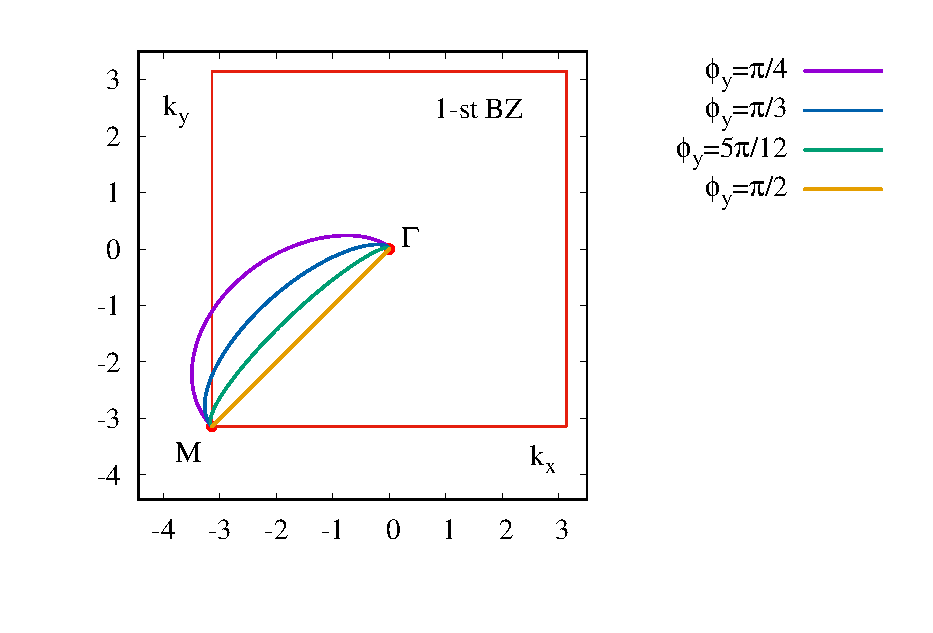
\includegraphics[width=0.7\linewidth]{Chapters/1_pi_pulse_tex/figure_c/3/Pulse_p.eps}} \\
\caption{Middle point trajectories of the momentum distribution for different phases between $X$ and $Y$ projections of the vector potential.}
\label{fig:Pulse_p_3}
\end{figure}

\begin{figure}[h!]
\begin{minipage}[h]{0.5\linewidth}
\center{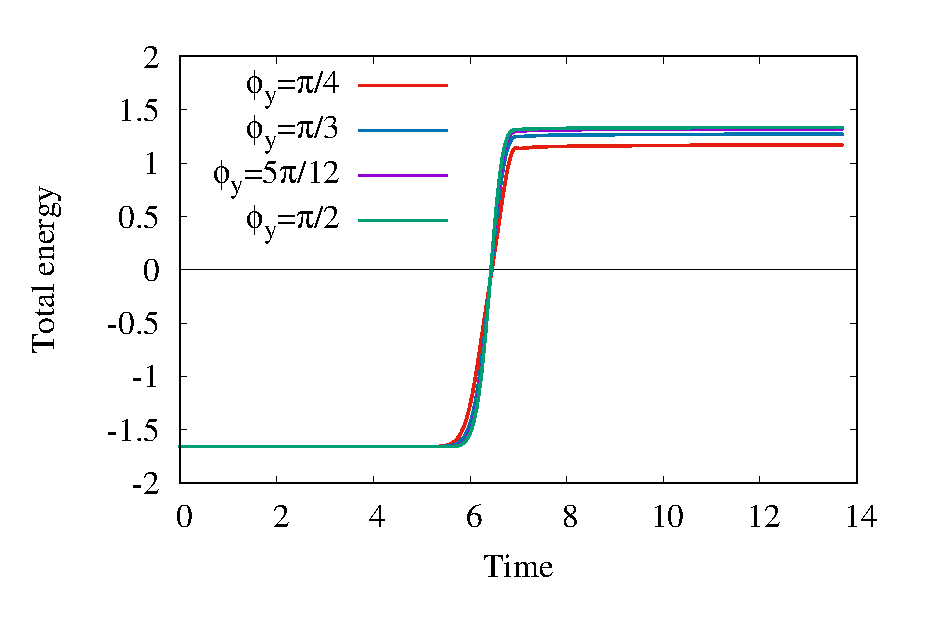
\includegraphics[width=1\linewidth]{Chapters/1_pi_pulse_tex/figure_c/3/Etot.eps}} (a) \\
\end{minipage}
\hfill
\begin{minipage}[h]{0.5\linewidth}
\center{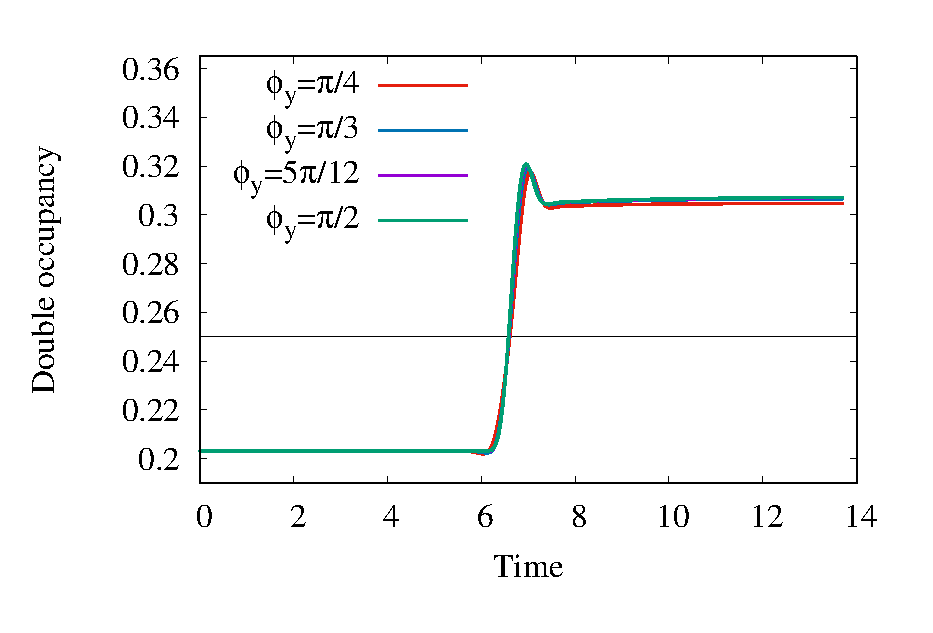
\includegraphics[width=1\linewidth]{Chapters/1_pi_pulse_tex/figure_c/3/docc.eps}} \\(b)
\end{minipage}
\caption{Dependence of the total energy (a) and double occupancy (b) for different phases between $X$ and $Y$ projections of the vector potential.}
\label{fig:Etot_3}
\end{figure}

To obtain a more significant population inversion better to apply the pulse with linear $XY$-polarization; this can be seen from the graph of the total energy in Fig.~\ref{fig:Etot_3}a. Gradually increasing the polarization from linear to circular, the final value of the total energy slightly decreases. But the double occupancy (Fig.~\ref{fig:Etot_3}b) react to the change of phase between the $X$ and $Y$ components of the field polarization not significantly.
\FloatBarrier

%\subsection{The frequency dependence}

Next, consider how the physical parameters of the model change under the action of half-cycle circularly polarized vector potentials with different frequencies. Figs.~\ref{fig:Pulses_2} shows the graphs vector potentials for these cases. 
\begin{figure}[h!]
\begin{minipage}[h]{0.5\linewidth}
\center{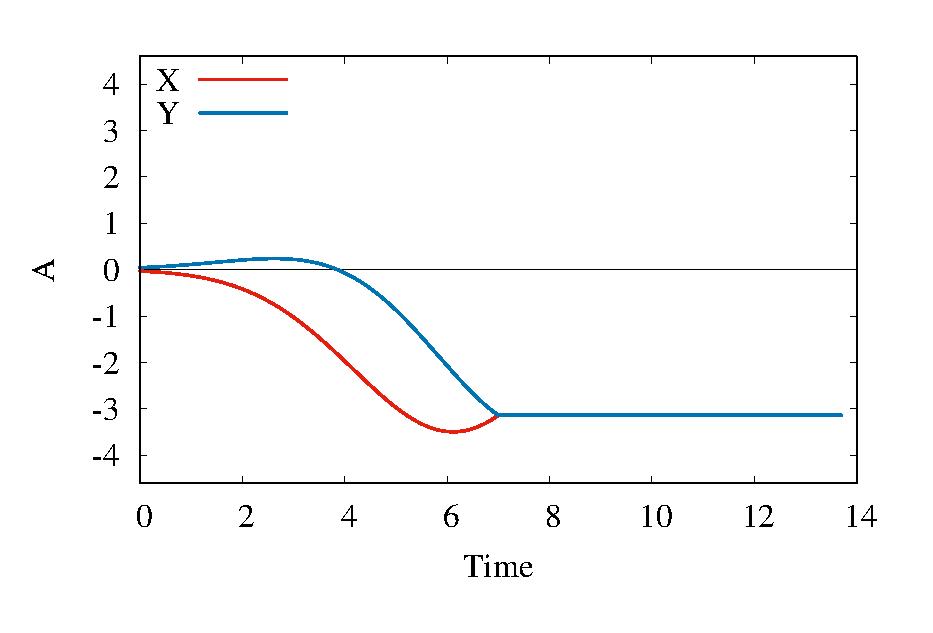
\includegraphics[width=1\linewidth]{Chapters/1_pi_pulse_tex/figure_c/2/Pulse_0.eps}} (a) \\
\end{minipage}
\begin{minipage}[h]{0.5\linewidth}
\center{\includegraphics[width=1\linewidth]{Chapters/1_pi_pulse_tex/figure_c/2/Pulse_4.eps}} \\(b)
\end{minipage}
\caption{Vector potentials with different frequencies: (a) $\omega=0.25$; (b) $\omega=2$.}
\label{fig:Pulses_2}
\end{figure}
%The trajectory of the momentum distribution is the same everywhere for each frequency. Than higher the frequency then faster the momentum distribution moves from the $\Gamma$ point of the Brillouin zone to M. 

Total energy and double occupancy respond strongly to such a frequency change (Fig.~\ref{fig:Etot_2}). The higher the frequency of the pulse, the greater the total energy and double occupancy, and therefore the greater the population inversion.
%\begin{figure}[h!]
%\center{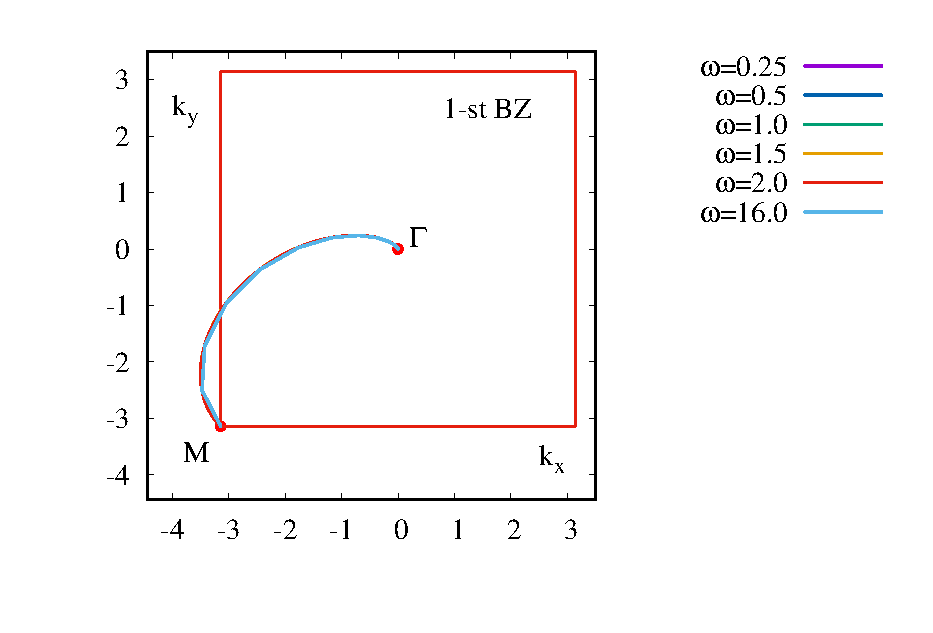
\includegraphics[width=0.7\linewidth]{Chapters/1_pi_pulse_tex/figure_c/2/Pulse_p.eps}} \\
%\caption{Middle point trajectories of the momentum distribution for different frequencies of the vector potential.}
%\label{fig:Pulse_p_2}
%\end{figure}
\begin{figure}[h!]
\begin{minipage}[h]{0.5\linewidth}
\center{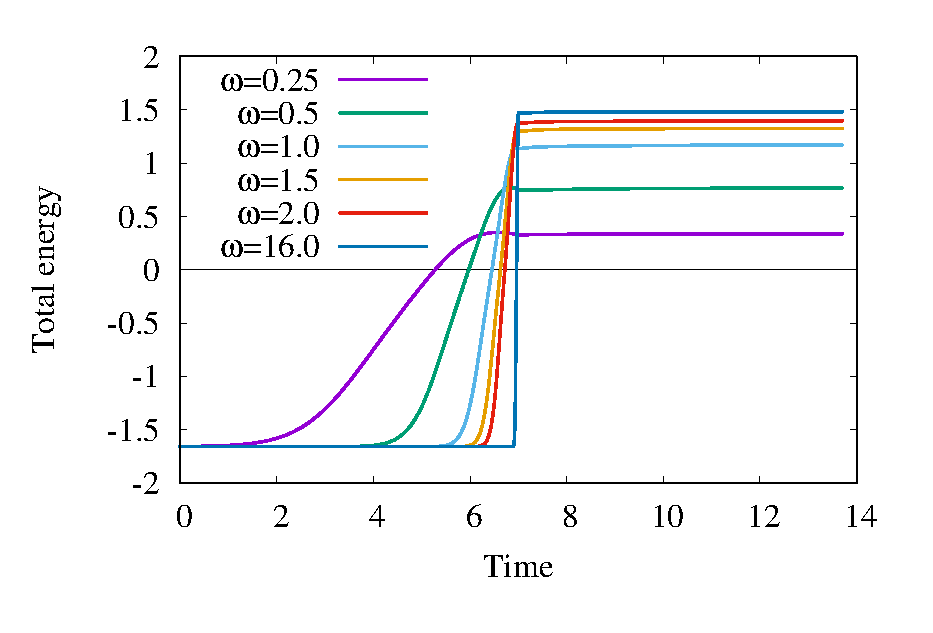
\includegraphics[width=1\linewidth]{Chapters/1_pi_pulse_tex/figure_c/2/Etot.eps}} (a) \\
\end{minipage}
\hfill
\begin{minipage}[h]{0.5\linewidth}
\center{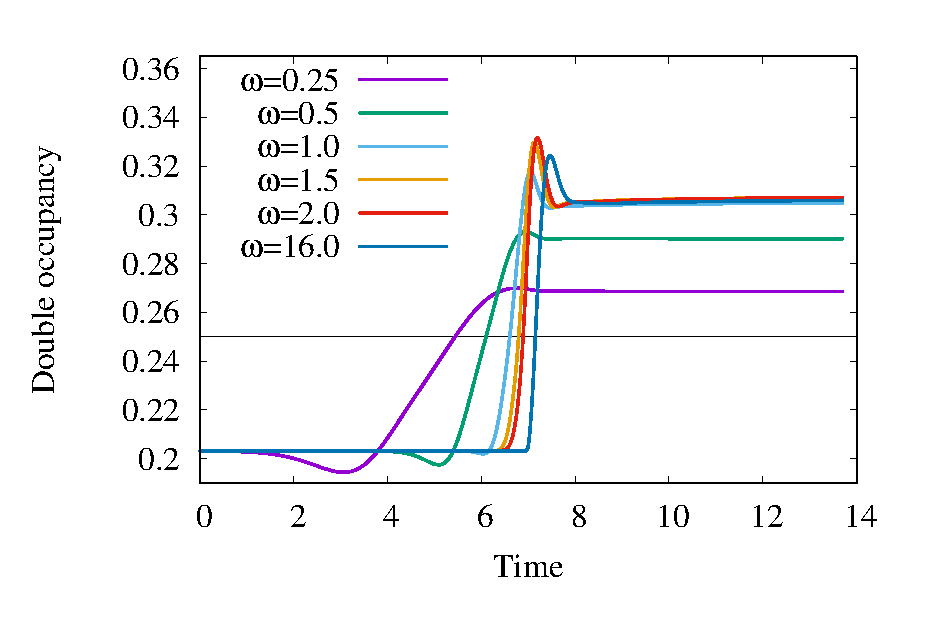
\includegraphics[width=1\linewidth]{Chapters/1_pi_pulse_tex/figure_c/2/docc.eps}} \\(b)
\end{minipage}
\caption{Dependence of the total energy (a) and double occupancy (b) from the frequency of the vector potential.}
\label{fig:Etot_2}
\end{figure}

In Figs.~\ref{fig:md_2} depicted the behavior of the momentum distribution in the circular field at different points in time for $U=2$. Distribution moves in the direction of the vector potential at $time=5.0$ to $time=7.0$ because electric field is switched on (Figs.~\ref{fig:md_2}a-d). After $time=7.0$ the distribution stop moving because process of relaxation starts and until $time=10.0$ the topology becomes smoother.
\begin{figure}[h!]
\begin{minipage}[h]{0.43\linewidth}
\begin{overpic}[width=1\textwidth]{Chapters/1_pi_pulse_tex/figure_c/2/A_550.jpg}
 \put (20,85) {(a)}
\end{overpic}
\end{minipage}
\hfill
\begin{minipage}[h]{0.43\linewidth}
\begin{overpic}[width=1\textwidth]{Chapters/1_pi_pulse_tex/figure_c/2/A_700.jpg}
 \put (20,85) {(d)}
\end{overpic}
\end{minipage}
\begin{minipage}[h]{0.43\linewidth}
\begin{overpic}[width=1\textwidth]{Chapters/1_pi_pulse_tex/figure_c/2/A_600.jpg}
 \put (20,85) {(b)}
\end{overpic}
\end{minipage}
\hfill
\begin{minipage}[h]{0.43\linewidth}
\begin{overpic}[width=1\textwidth]{Chapters/1_pi_pulse_tex/figure_c/2/A_750.jpg}
 \put (20,85) {(e)}
\end{overpic}
\end{minipage}
\begin{minipage}[h]{0.43\linewidth}
\begin{overpic}[width=1\textwidth]{Chapters/1_pi_pulse_tex/figure_c/2/A_650.jpg}
 \put (20,85) {(c)}
\end{overpic}
\end{minipage}
\hfill
\begin{minipage}[h]{0.43\linewidth}
\begin{overpic}[width=1\textwidth]{Chapters/1_pi_pulse_tex/figure_c/2/A_1000.jpg}
 \put (20,85) {(f)}
\end{overpic}
\end{minipage}
\caption{Momentum distribution for $U=2$ in different $time$ $\in$ [5.5,10] with $\omega=1$ and FWHM=1.}
\label{fig:md_2}
\end{figure}

\FloatBarrier

%\subsection{Circular monocycle pulse with different initial phases.}

Consider how the properties of the Hubbard model change under the influence of monocycle pulses at different values of the initial phase (Fig.~\ref{fig:Pulses_1}).
\begin{figure}[h!]
\begin{minipage}[h]{0.5\linewidth}
\center{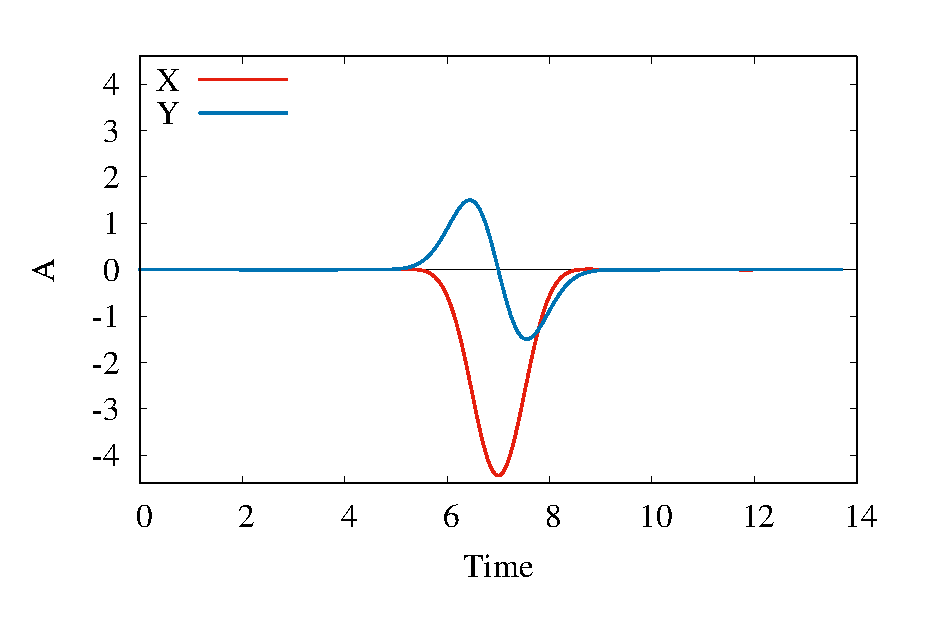
\includegraphics[width=1\linewidth]{Chapters/1_pi_pulse_tex/figure_c/1/u_0/Pulse_1.eps}} (a) \\
\end{minipage}
\hfill
\begin{minipage}[h]{0.5\linewidth}
\center{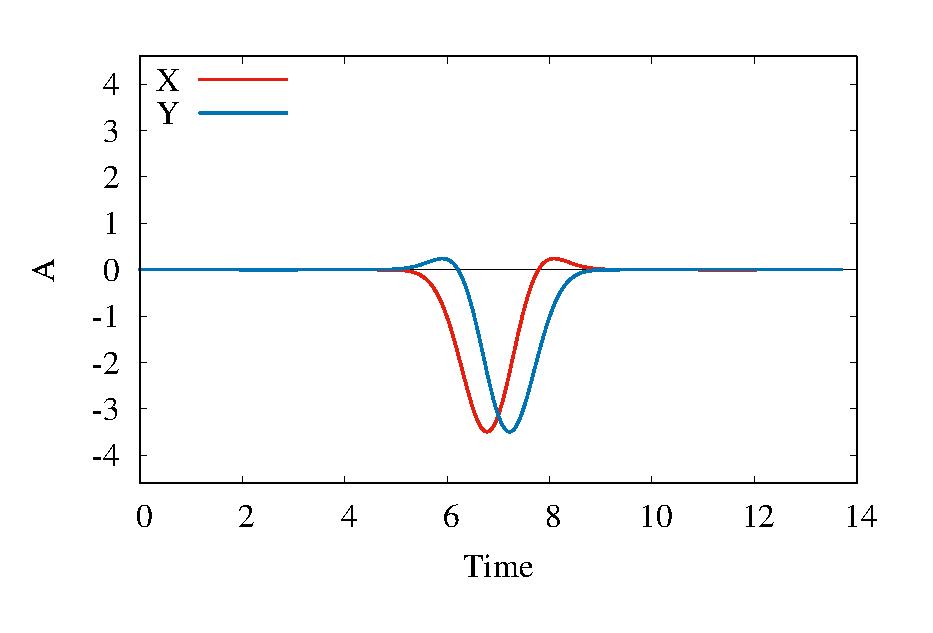
\includegraphics[width=1\linewidth]{Chapters/1_pi_pulse_tex/figure_c/1/u_0/Pulse_3.eps}} \\(c)
\end{minipage}
\begin{minipage}[h]{0.5\linewidth}
\center{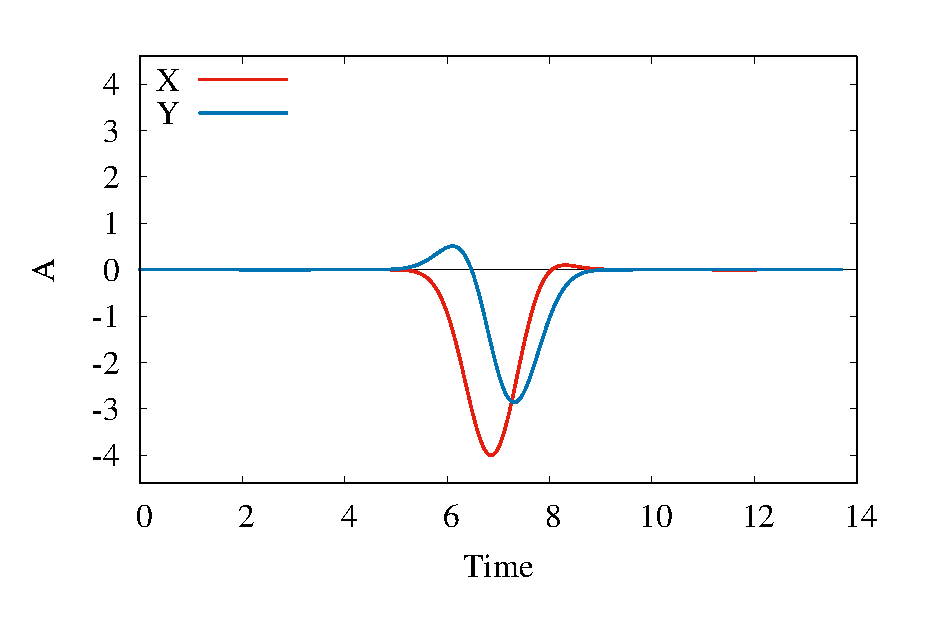
\includegraphics[width=1\linewidth]{Chapters/1_pi_pulse_tex/figure_c/1/u_0/Pulse_2.eps}} (b) \\
\end{minipage}
\hfill
\begin{minipage}[h]{0.5\linewidth}
\center{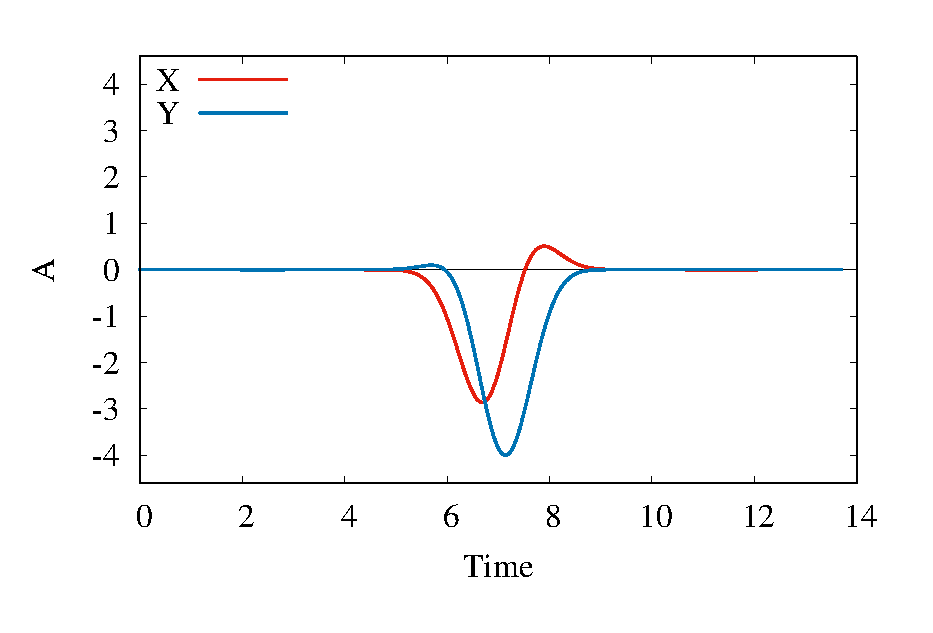
\includegraphics[width=1\linewidth]{Chapters/1_pi_pulse_tex/figure_c/1/u_0/Pulse_4.eps}} \\(d)
\end{minipage}
\caption{Vector potentials with different initial phases: (a) $\phi_y=0$; (b) $\phi_y=\pi /6$; (c) $\phi_y=\pi /4$; (d) $\phi_y=\pi /3$.}
\label{fig:Pulses_1}
\end{figure}

Moving the maximum of the momentum distribution from $\Gamma$ point of the Brillouin zone to the M point is depicted in Fig.~\ref{fig:Pulse_p_1}. 

Figs.~\ref{fig:Etot_1} shows the total energy and double occupancy for different values of the initial phases of the vector potential and for various Coulomb interactions $U$. Fig.~\ref{fig:Etot_1}a depicts the total energy for a pulse at $U=0$. The maximum value of the total energy is reached for $\phi_y=\pi /4$. The total energy for $\phi_y=\pi /6$ and $\phi_y=\pi /3$ are symmetrical relative to the middle of the pulse ($time=7$) and graph for $\phi_y=0$ symmetrical since it is always equidistant from M points of the Brillouin zone during the whole pulse time (Fig.~\ref{fig:Pulse_p_1} red line). The double occupancy (Fig.~\ref{fig:Etot_1}a) is equal to $0.25$ during all time, which must be in case of $U=0$.


\begin{figure}[h!]
\center{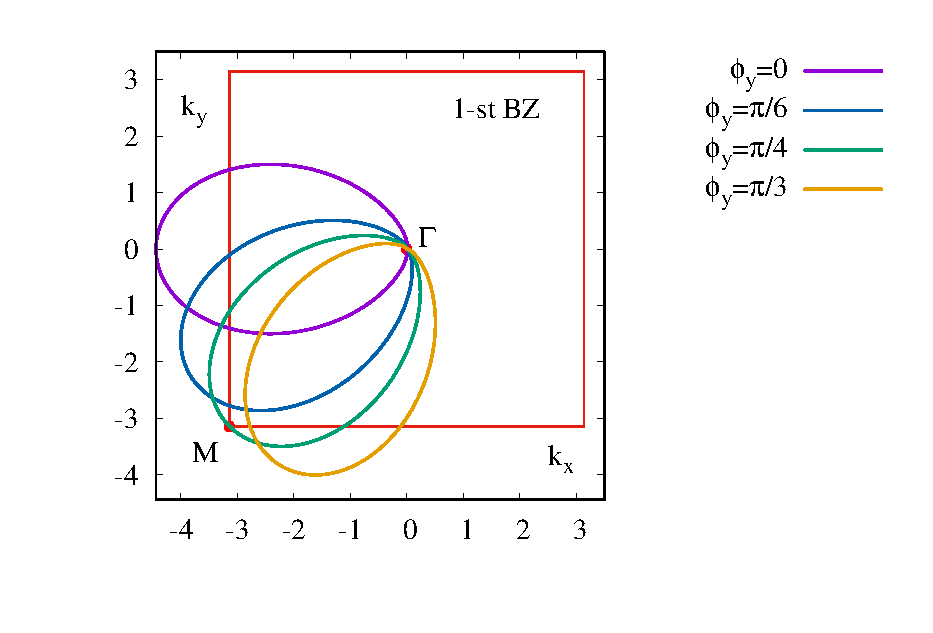
\includegraphics[width=0.7\linewidth]{Chapters/1_pi_pulse_tex/figure_c/1/u_0/Pulse_p.eps}} \\
\caption{Middle point trajectories of the momentum distribution with different initial phases of the vector potential.}
\label{fig:Pulse_p_1}
\end{figure}
Figs. \ref{fig:Etot_1}b,d show the total energy and double occupancy for a monocycle pulse at different initial phases in the case of $U=2$. The symmetry of the total energy with respect to the middle of the pulse disappears gradually depending on the magnitude of interaction.

All considered pulses lead to population inversion. The total energy for $\phi_y=\pi /6$ and $\phi_y=\pi /3$ are not any more symmetrical relative to the middle of pulse $time=7$. The curve at $\phi_y=\pi /6$ has a bigger maximum of the total energy comparing to $\phi_y=\pi /3$. Increasing the interaction lead to increasing of an energy absorption by the system and thus it increases the temperature during the pulse. The temperature rise makes the flatter momentum distribution that reduces the value of the population inversion, because more electrons are now may extend to the edges of the "hat" of the momentum distribution. At the same time, as it shown by previous calculations, the form of the "hat" of the momentum distribution for the correlated system itself may vary during the pulse. Thus, competition of the effects: inclusion of correlations that tend to bend the "hat" of the momentum distribution, shifting the momentum distribution by the vector potential to a more "favorable" position and heating the system, may explain why we see the maximum value of the total energy and double occupancy for the pulse with $\phi_y=\pi /3$ slightly larger than for $\phi_y=\pi /4$ in Figs.~\ref{fig:Etot_1}b,d.
\begin{figure}[h!]
\begin{minipage}[h]{0.5\linewidth}
\center{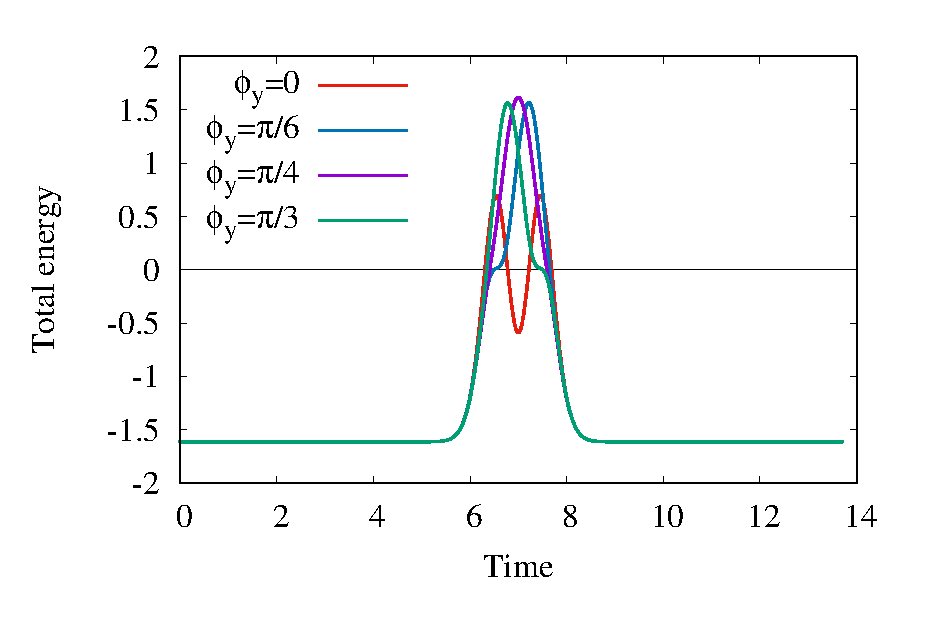
\includegraphics[width=1\linewidth]{Chapters/1_pi_pulse_tex/figure_c/1/u_0/Etot.eps}} (a) \\
\end{minipage}
\hfill
\begin{minipage}[h]{0.5\linewidth}
\center{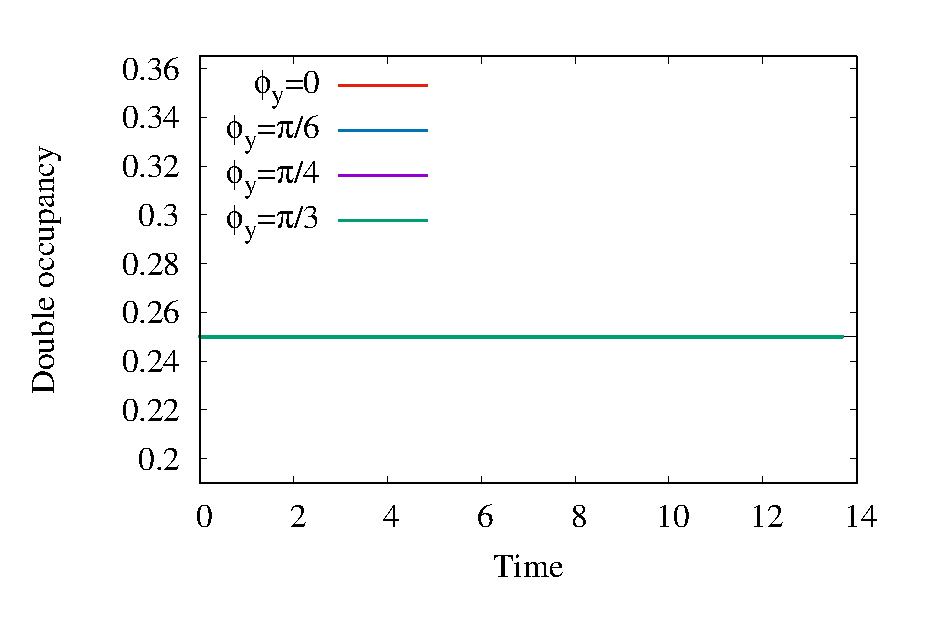
\includegraphics[width=1\linewidth]{Chapters/1_pi_pulse_tex/figure_c/1/u_0/docc.eps}} \\(c)
\end{minipage}
\begin{minipage}[h]{0.5\linewidth}
\center{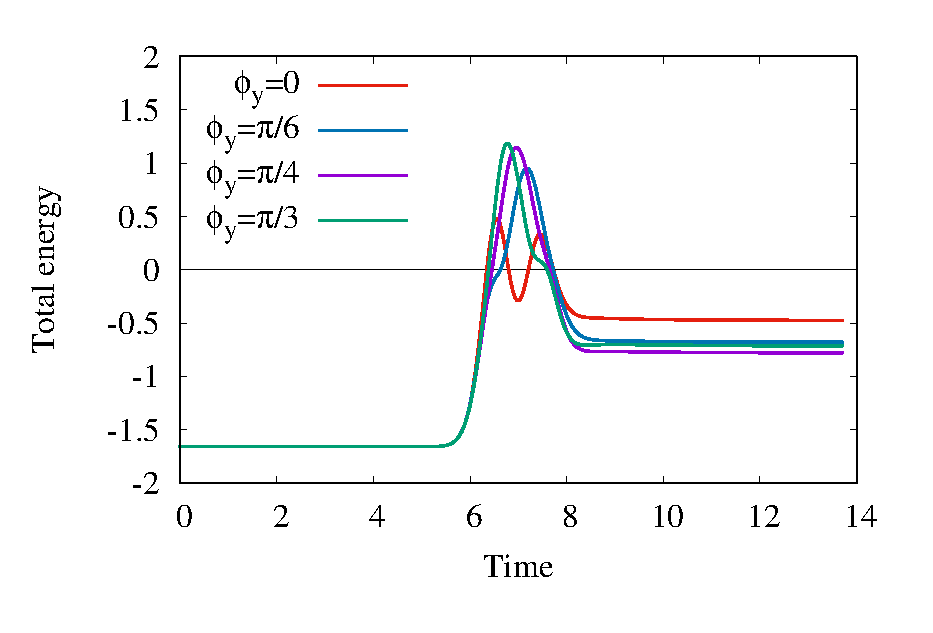
\includegraphics[width=1\linewidth]{Chapters/1_pi_pulse_tex/figure_c/1/u_2/Etot.eps}} (b) \\
\end{minipage}
\hfill
\begin{minipage}[h]{0.5\linewidth}
\center{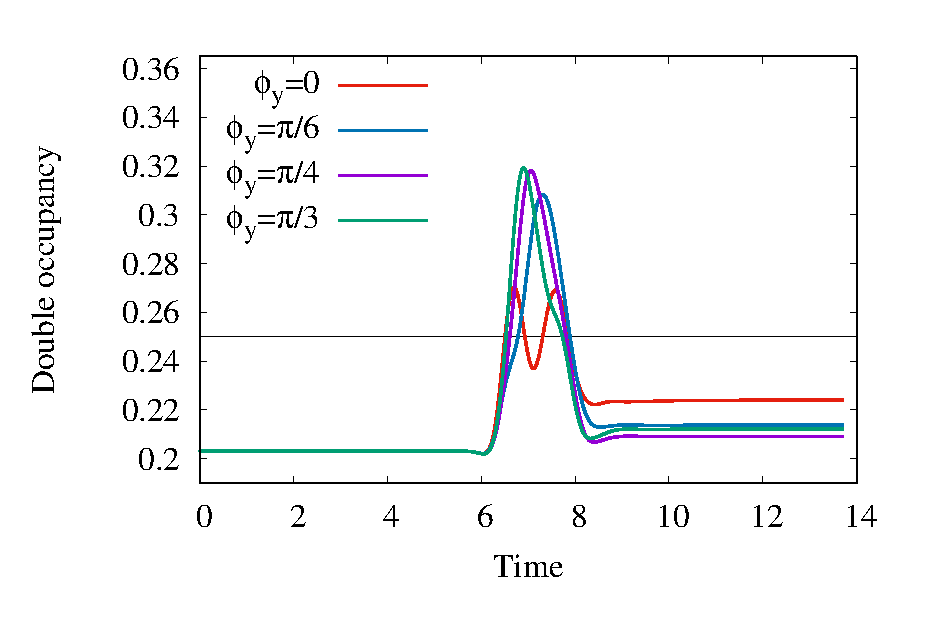
\includegraphics[width=1\linewidth]{Chapters/1_pi_pulse_tex/figure_c/1/u_2/docc.eps}} \\(d)
\end{minipage}
\caption{Dependence of total energy and double occupancy from different initial phases of the vector potential: (a),(c) case of $U=0$; (b),(d) case of $U=2$.}
\label{fig:Etot_1}
\end{figure}

\FloatBarrier

\subsection{Beyond of monocycle condition}

It is interesting to explore how the model behaves outside of the monocycle condition. Fig.~\ref{fig:Pulses_4} shows the graphs of half-cycle circularly polarized vector potentials with different ratios FWHM and $\omega$.
\begin{figure}[h!]
\begin{minipage}[h]{0.5\linewidth}
\center{\includegraphics[width=1\linewidth]{Chapters/1_pi_pulse_tex/figure_c/4/Pulse_1.eps}} (a) \\
\end{minipage}
\hfill
\begin{minipage}[h]{0.5\linewidth}
\center{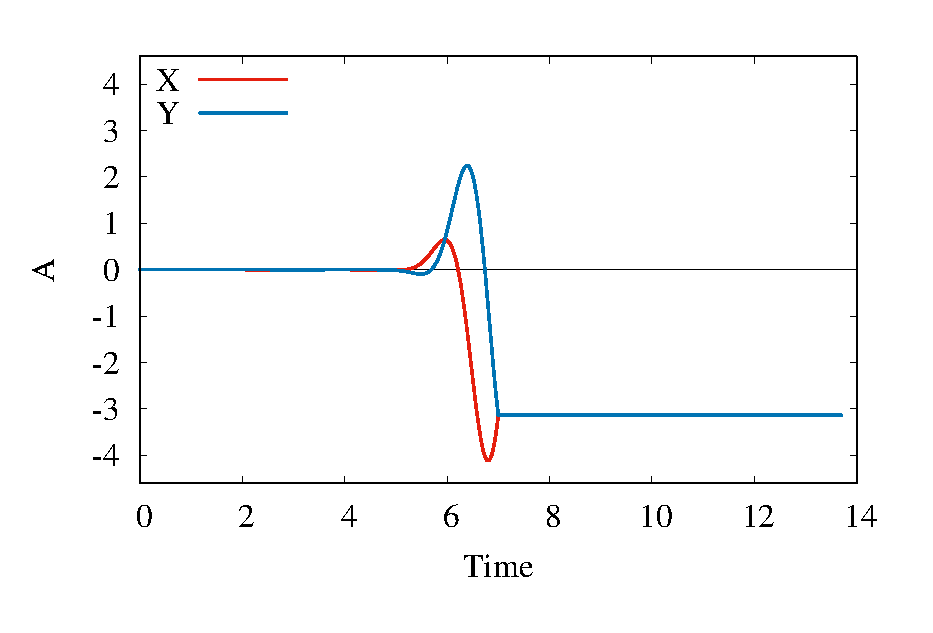
\includegraphics[width=1\linewidth]{Chapters/1_pi_pulse_tex/figure_c/4/Pulse_3.eps}} \\(c)
\end{minipage}
\begin{minipage}[h]{0.5\linewidth}
\center{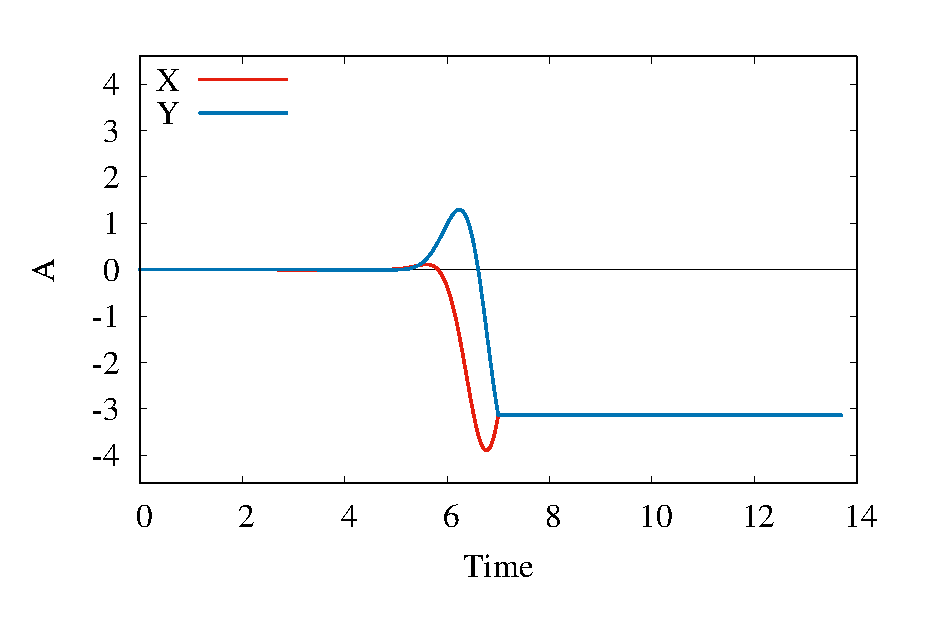
\includegraphics[width=1\linewidth]{Chapters/1_pi_pulse_tex/figure_c/4/Pulse_2.eps}} (b) \\
\end{minipage}
\hfill
\begin{minipage}[h]{0.5\linewidth}
\center{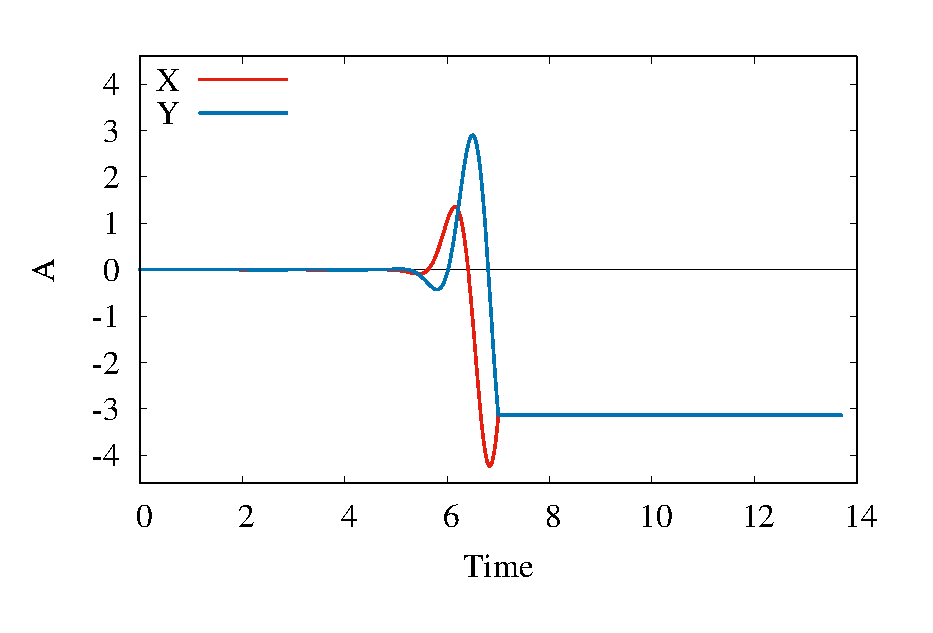
\includegraphics[width=1\linewidth]{Chapters/1_pi_pulse_tex/figure_c/4/Pulse_4.eps}} \\(d)
\end{minipage}
\caption{Vector potentials for different frequencies with fixed FWHM: (a) $\omega=1.0$ monocycle condition; (b) $\omega=2.0$; (c) $\omega=3.0$; (d) $\omega=4.0$.}
\label{fig:Pulses_4}
\end{figure}

By increasing the frequency of the pulse and leaving the FWHM constant we move away from the monocycle condition Eq.~\eqref{eq:monocycle_condition}. Fig.~\ref{fig:Pulse_p_4} illustrate trajectory of the center momentum distribution for $\pi$-pulse. Line with $\omega=1$ is a half-cycle pulse with the monocycle condition.
\begin{figure}[h!]
\center{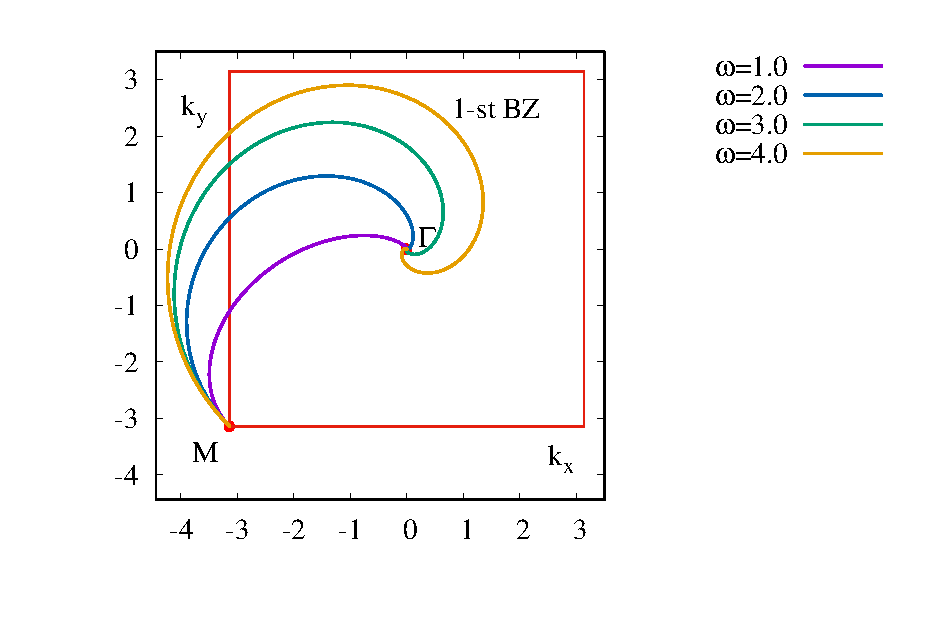
\includegraphics[width=0.7\linewidth]{Chapters/1_pi_pulse_tex/figure_c/4/Pulse_p.eps}} \\
\caption{Middle point trajectories of the momentum distribution for different frequencies with fixed FWHM of the vector potentials.}
\label{fig:Pulse_p_4}
\end{figure}

The total energy of such pulses (Fig.~\ref{fig:Etot_4}a) has a different structure during the excitation, nevertheless the optimal inversion presented at the $\pi$-pulse with the monocycle condition. This can be explained by the fact that the monocycle condition has the shortest way to move the center of momentum distribution from $\Gamma$ to M point, which contributes to less heating of the system. 
\begin{figure}[h!]
\begin{minipage}[h]{0.5\linewidth}
\center{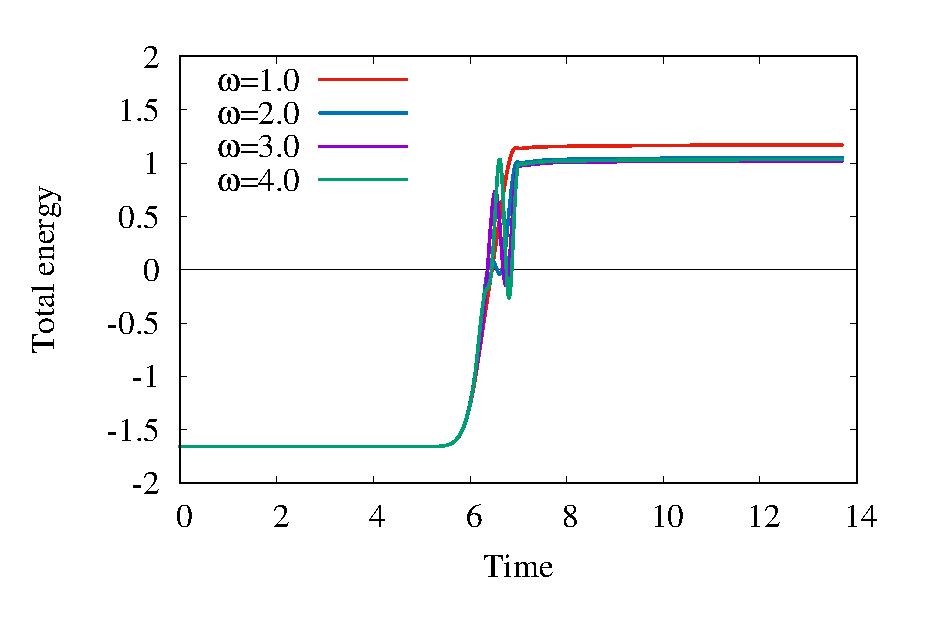
\includegraphics[width=1\linewidth]{Chapters/1_pi_pulse_tex/figure_c/4/Etot.eps}} (a) \\
\end{minipage}
\hfill
\begin{minipage}[h]{0.5\linewidth}
\center{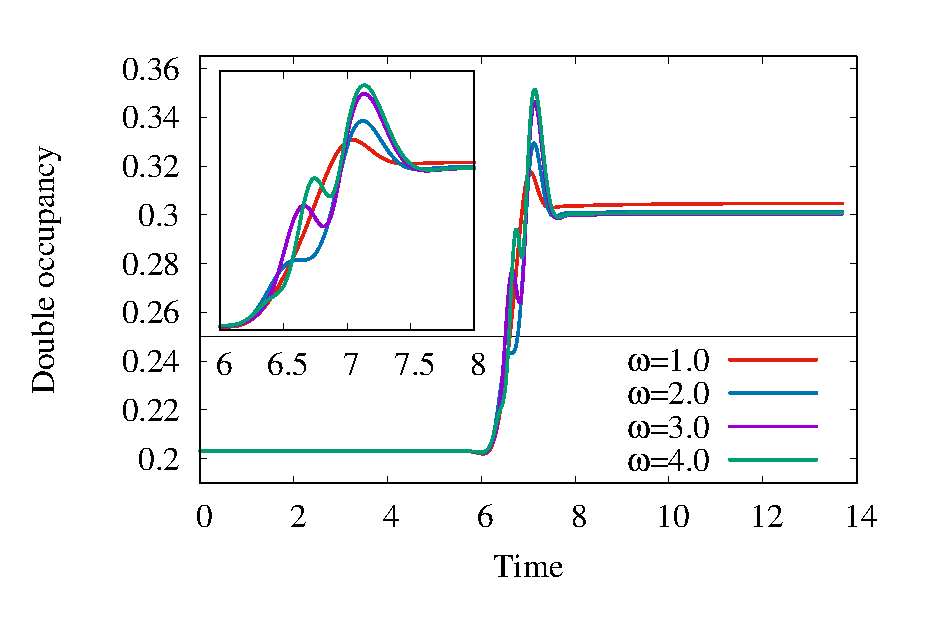
\includegraphics[width=1\linewidth]{Chapters/1_pi_pulse_tex/figure_c/4/docc.eps}} \\(b)
\end{minipage}
\caption{Dependence of the total energy (a) and double occupancy (b) from different frequencies with fixed FWHM of the vector potentials.}
\label{fig:Etot_4}
\end{figure}

Beyond of the monocycle condition Eq. \eqref{eq:monocycle_condition}  additional peak appears in the graphs of total energy and double occupancy (Fig.~\ref{fig:Etot_4}). The peak gradient increases and moves towards greater times. The presence of the peak at these graphs is due to the fact that the center of momentum distribution in the non-monocycle case passes near another M point in the first Brillouin zone, thereby creating an inversion on that part of the trajectory. 

\FloatBarrier

\subsection{Multicycle pulse}

In this part, we discuss how to create a maximum population inversion during multicycle circularly polarized pulse. A ramp of the vector potential is depicted in Fig.~\ref{fig:Pulses_5}. The maximum amplitude of the vector potential is $A_{max}=4.44$. 
\begin{figure}[h!]
\center{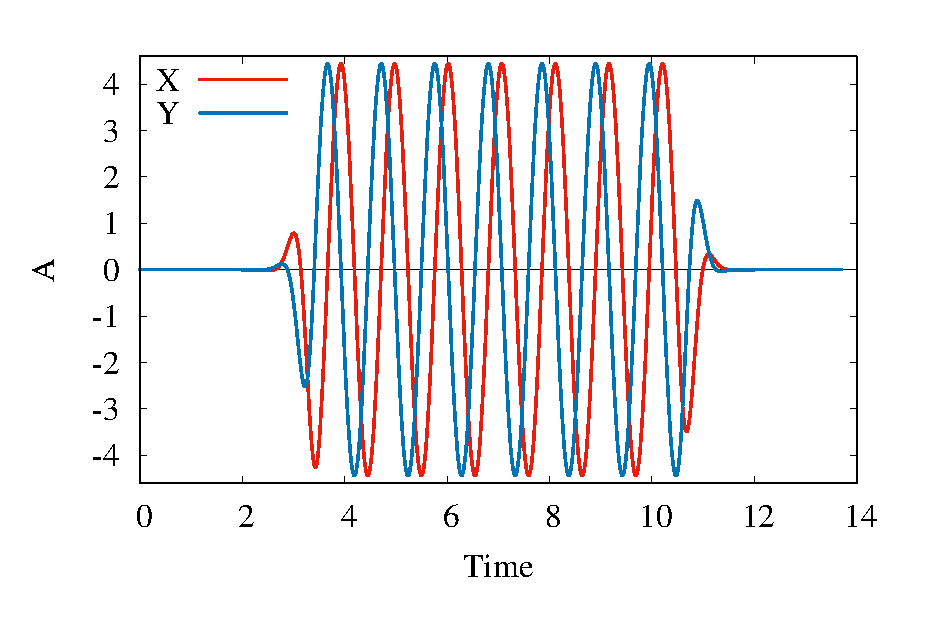
\includegraphics[width=0.55\linewidth]{Chapters/1_pi_pulse_tex/figure_c/plot/Pulse_3.eps}} \\
\caption{The ramp of the multicycle circularly polarized vector potential.}
\label{fig:Pulses_5}
\end{figure}

This form of vector potential that moves the middle of the momentum distribution from $\Gamma$ through all four M points in the 2D square lattice in Brillouin zone (Fig. \ref{fig:Pulse_p_5}).
\begin{figure}[h!]
\center{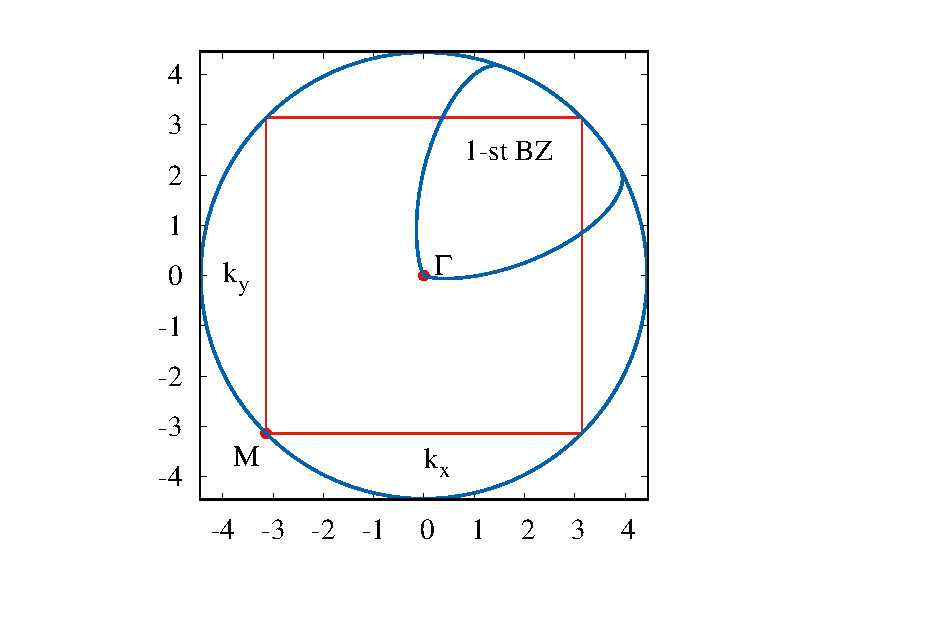
\includegraphics[width=0.7\linewidth]{Chapters/1_pi_pulse_tex/figure_c/plot/Pulse_p_w1.eps}} \\
\caption{Middle point trajectories of the momentum distribution induced by the ramp of the multicycle circularly polarized vector potential.}
\label{fig:Pulse_p_5}
\end{figure}

The corresponding total energy and double occupancy are shown in Fig.~\ref{fig:Etot_5}. General patterns characterize results for all frequencies. Initially, the total energy increases from negative to positive value, then oscillates and finally decreases to the negative. The behavior of the double occupancy is very similar, except that it can only be positive and grows to a higher value than 0.25.
This corresponds to the fact that the maximum of the momentum distribution first goes from the $\Gamma$ point to a circle close to the M point (Fig.~\ref{fig:Pulse_p_5}). Moving in a circle near all four M points inversion of the population occurs, and over the X and Y points in the BZ it disappears. 

\clearpage

\begin{figure}[h!]
\begin{minipage}[h]{0.5\linewidth}
\begin{overpic}[width=1\textwidth]{Chapters/1_pi_pulse_tex/figure_c/plot/Etot_1.eps}
 \put (22,55) {(a)}
\end{overpic}
\end{minipage}
\hfill
\begin{minipage}[h]{0.5\linewidth}
\begin{overpic}[width=1\textwidth]{Chapters/1_pi_pulse_tex/figure_c/plot/docc_1.eps}
 \put (24,55) {(d)}
\end{overpic}
\end{minipage}
\begin{minipage}[h]{0.5\linewidth}
\begin{overpic}[width=1\textwidth]{Chapters/1_pi_pulse_tex/figure_c/plot/Etot_2.eps}
 \put (22,55) {(b)}
\end{overpic}
\end{minipage}
\hfill
\begin{minipage}[h]{0.5\linewidth}
\begin{overpic}[width=1\textwidth]{Chapters/1_pi_pulse_tex/figure_c/plot/docc_2.eps}
 \put (24,55) {(e)}
\end{overpic}
\end{minipage}
\begin{minipage}[h]{0.5\linewidth}
\begin{overpic}[width=1\textwidth]{Chapters/1_pi_pulse_tex/figure_c/plot/Etot_3.eps}
 \put (22,55) {(c)}
\end{overpic}
\end{minipage}
\hfill
\begin{minipage}[h]{0.5\linewidth}
\begin{overpic}[width=1\textwidth]{Chapters/1_pi_pulse_tex/figure_c/plot/docc_3.eps}
 \put (24,55) {(f)}
\end{overpic}
\end{minipage}
%\begin{minipage}[h]{0.5\linewidth}
%\begin{overpic}[width=1\textwidth]{Chapters/1_pi_pulse_tex/figure_c/%plot/Etot_4.eps}
% \put (22,55) {(d)}
%\end{overpic}
%\end{minipage}
%\hfill
%\begin{minipage}[h]{0.5\linewidth}
%\begin{overpic}[width=1\textwidth]{Chapters/1_pi_pulse_tex/figure_c/%plot/docc_4.eps}
% \put (24,55) {(h)}
%\end{overpic}
%\end{minipage}
\caption{Dependence of the total energy (a-c) left column and corresponded double occupancy (d-f) right column, at $U=2$ from different frequencies ($\omega=1$;$3$ and $6$) of the multicycle circularly polarized vector potential.}
\label{fig:Etot_5}
\end{figure}
And finally, at the end of the pulse, the maximum of distribution returns to its initial location at the $\Gamma$ point, but it has already been changed by the effects of correlations, external field, and temperature.
As the pulse frequency increases, the total energy tends to oscillate and be in the majority with a positive value. The higher the field frequency, the longer it remains in transient positive value. The double occupancy fully arrives above 0.25 at the time of the excitations for frequencies above $\omega=1$. 

The total energy and double occupancy at high frequencies of the external field initially have a change in the amplitude of oscillations. However, after some time, the mean value and amplitude of oscillations hardly change. This implies that we detect a transition to a mode where physical observables are periodic in time what can be connected with the Floquet regime.

%\vspace{5mm} %5mm vertical space
\FloatBarrier
\section{Summary}
Thus, summarizing the various options for changing the sign of the interaction in the Hubbard model under the influence of the external field, we come to the following conclusions:

1. Creating of the population inversion becomes more efficient in linear pulse compare to circularly polarized (Fig.~\ref{fig:Etot_3}a).

2. Higher pulse frequency helps to significantly increase inversion in the case of $\pi$-pulse (Fig.~\ref{fig:Etot_2}).

3. With the circularly polarized vector potential, the maximum positive value of the total energy depends on the initial phase as well. To create population inversion, do not necessary to have a phase due to which the middle of momentum distribution is transferred exactly from the $\Gamma$ point to M, as previously expected. This case is shown in Fig.~\ref{fig:Etot_1}b.

4. Moving away from the monocycle condition for circular polarization allows creating controlled peaks of the total energy that can change the sign of the interaction (Fig.~\ref{fig:Etot_4}a).

5. It is important to note how the parameters of the system and the pulse separately affect the distribution. In equilibrium, correlations and temperature blur the Fermi step, the electric field used as a vector potential shift the distribution by the value of this vector potential. In nonequilibrium in the absence of correlations, the momentum distribution moves in the direction of the vector potential without changing its shape. 
The momentum distribution distorted under the action of the combined effects of correlations, the electric field (for all considered polarization) and an increasing of the effective temperature.
\clearpage
\bibliographystyle{abbrvnat}
\bibliography{references}
\end{document}
